%%%%%%%%%%%%%%%%%%%%%%%%%%%%%%%%%
% 7CCS4PRJ Final Year Individual Project Report
% konstantin.draganov@kcl.ac.uk
%%%%%%%%%%%%%%%%%%%%%%%%%%%%%%%%%
\documentclass[11pt]{informatics-report}
\usepackage{color}
\usepackage[square,sort,comma,numbers]{natbib} %References
\usepackage{placeins}
\usepackage{amsmath}

%%%%%%%%%%%%%%%%%%%%%%%%%%%%%%%%%
% Front Matter - project title, name, supervisor name and date
%%%%%%%%%%%%%%%%%%%%%%%%%%%%%%%%%
\reportTitle{7CCS4PRJ Final Year Individual Project}
\projectTitle{iBus Disruption Monitor}
%\projectTitle{Real-Time Visualisation of Bus Delays in London using AVL Data}
\productTitle{Real-Time Visualisation of Bus Delays in London using AVL Data}
%\productTitle{iBus Disruption Monitor}
\subtitle{A project in collaboration with Transport for London}
\author{Konstantin Vladimirov Draganov}
\studentID{1101314}
\supervisor{Dr Steffen Zschaler}
\date{September 2014 - April 2015}
\wordCount{}
\abstractFile{FrontMatter/abstract.tex}
\ackFile{FrontMatter/acknowledgements.tex} %Remove line if you do not want acknowledgements

\begin{document}
\createFrontMatter
\onehalfspacing
\tableofcontents
\doublespacing

%%%%%%%%%%%%%%%%%%%%%%%%%%%%%%%%%
% Report Content
%%%%%%%%%%%%%%%%%%%%%%%%%%%%%%%%%
%The central part of the report usually consists of three or four chapters detailing the technical work undertaken during the project. {\bf{\textcolor{red}{The structure of these chapters is highly project dependent}}}. They can reflect the chronological development of the project, e.g. design, implementation, experimentation, optimisation, evaluation, etc (although this is not always the best approach). However you choose to structure this part of the report, you should make it clear how you arrived at your chosen approach in preference to other alternatives. In terms of the software that you produce, you should describe and justify the design of your programs at some high level, e.g. using OMT, Z, VDL, etc., and you should document any interesting problems with, or features of, your implementation. Integration and testing are also important to discuss in some cases. You may include fragments of your source code in the main body of the report to illustrate points; the full source code is included in an appendix to your written report.

%NEED TO INCLUDE OPTIMISATIONS THAT COULD BE APPLIED

%The report should answer the following questions:
%What is the problem
%Here is how we can solve it
%Here are the benefits
%Here is the evidence that we solved it

%Everything in the report should be there for a reason (supporting and building other sections)
%This is one of the most important components of the report. It should begin with a clear statement of what the project is about so that the nature and scope of the project can be understood by a lay reader. It should summarise everything that you set out to achieve, provide a clear summary of the project's background and relevance to other work, and give pointers to the remaining sections of the report, which will contain the bulk of the technical material \cite{einstein}.
\chapter{Introduction}
%\section{Motivation}
London bus network is one of the largest and most advanced bus networks in the world. It is responsible for more than 2.4 billion passenger journeys a year \cite{TFL1}. The constant population growth of England's capital has been also driving the expansion and improvement of the transport networks across the city \cite{TFL2}.This leads to more pressure being put on the infrastructure which includes not only the road network and the bus fleet, but on the technological systems that aid its operation as well.
%The capital's bus network is continually expanding along with the city's population \cite{TFL2}.

Transport for London (TFL) is in charge of its operation and its bus network is recognised as one of the top in the world in terms or reliability, affordability and cost-effectiveness \cite{TFL1}. Maintaining such a large scale network requires careful planing and monitoring. Being able to operate such a high reliability service 24/7 364 days in the year, requires employing new technologies. This also helps keep costs down and therefore makes the service more affordable and accessible for the general travelling public. 

Each bus in the TFL network is equipped with state of the art GPS enabled automatic vehicle location (AVL) system named iBus\cite{ibusdeployment}. This AVL system has led to improved fleet management and has enabled the creation and improvement of multiple applications \cite{eps354267}. The system is generating large sets of both real-time and historical data, which aids the bus operators and the emergency control room at TFL, responsible for maintaining the bus network (CentreComm), to better manage and maintain the smooth operation of the bus network. This includes both planning for future demand and growth, as well as emergencies and innervation during the daily operation of the network. 

However, there are still some situations and problems which require CentreComm staff to carry out manual analysis of the available data. This means that there is lack of readily available preprocessed information. Having to manually monitor thousands of buses continuously is very impractical. That is the reason why currently CentreComm operators rely heavily on individual bus operators and drivers to alert them of possible problems. Once alerted about a potential disruptions in the network, they (CentreComm) can start their own investigation - first verifying what they have been told by the bus drivers/operators and then into finding the cause and the actual severity of the problem. This could often result in time and resources being spent (wasted) on investigating non existent problems. Worse, it often leads to time and resources being spend on investigating and dealing with problems of less importance than others, because of wrong interpretation (exaggeration) by bus drivers and/or operators involved in these situations. This project tries to address these inefficiencies and to propose a prototypical tool for real-time monitoring of the bus delays in London's bus network.

%This is where this project comes in place to address this inefficiency and to propose, implement and evaluate a prototypical tool for real time monitoring of the bus network.
%This way of operation however often leads to some less important problems being treated with higher priority over some actually more important ones. 
%Having to spend time to manually work through hundreds lines of information is very impractical, time consuming and error prone.
%However there are currently problems for which CentreComm staff are required to manually analyse these data sets in order to discover in which parts of the networks problems are occurring.
%This is because there is lack of readily available preprocessed information. 
%This is very impractical and time consuming and currently they ultimately rely on individual bus operators and drivers to notify them of possible problems. 
%Once alerted of a possible disruption in the network they can start their own investigation first verifying what they have been told by the bus drivers/operators and then into finding the cause and the actual severity of the problem. This often could lead to spending time and resources into investigating non existent problems. This is where this project comes in place to address this inefficiency and to propose, implement and evaluate a prototypical tool for real time monitoring of the bus network.

%This seems an odd mix. Some of these are product requirements, 
%some seem more like tasks that you will need to do to satisfy these requirements. Perhaps worth restructuring? Think about the overall aim, objectives supporting this aim, and finally actions to take to achieve the objectives.

%Project scope is the part of project planning that involves determining and documenting a list of specific project goals, deliverables, tasks, costs and deadlines.
\section{Scope}
The scope of this project is to analyse the current work flow of CentreComm operators and their needs. The main goal is to design and implement a prototype which to automate and improve the work flows currently in place. This tool has to work and analyse the data that has been made available by TFL. This analysis is required to happen in real time as more data is being made available. The reason for this being that it would be used as an objective source of information for the delays in the bus network at each point in time. In addition to this, the project needs to perform analysis of what visualisation will be useful, suitable and usable for the output.

%The four main problems that are in the scope of this project and need to be solved are:
%\begin{itemize}
%	\item Analysing and identifying the disruptions in the bus network in real-time using the provided data.
%	\item Producing a prioritised list of the disruptions classified using rules and heuristics gathered during meetings and discussions with the key stakeholders from TFL.
%	\item Visualising the calculated list in an appropriate format.
%	\item Evaluating the performance of the tool. This is essential as it need to be proven that the results could be trusted.
%\end{itemize} 

\section{Aims}
The main aim of this project is to design and implement a real-time visualisation tool which will be used highlight disrupted routes or parts of the TFL bus network which experience delays. Potentially, the system could alert (be proactive) of possible delays even before the bus drivers or operators have noticed and contacted CentreComm for assistance. This aim could be subdivided into two smaller aims:
\begin{itemize}
	\item The first one, which is independent of the other, is to enable the processing of the data generated by the buses in the TFL's bus network. The tool needs to be able to analyse the input data sets, calculate and output a list of the disruption that are observed in the network. It has to present information regarding the location (route section) in the transport network and their severity.
	\item The second part of the main aim is to visualise the generated output in a way that is easy to use and understand. It is also important to note that the visualisation should be capable of updating itself whenever the list of delays have changed. This needs to happen in real time as well.
\end{itemize}
%In addition to the above aims the project has to evaluate the tool that is developed.

%	1. Are broad statement of the desired outcome, or general intentions of the project
%	2. Emphasize what is to be accomplished (not how it is to be accomplished)
%	3. Address the long-term project outcomes
\section{Objectives}
The objectives that have been followed in order to successfully meet the above stated aims are:
\begin{itemize}
	\item Obtain an in depth understanding of the problem and current work-flows that are in place at CentreComm.
	\item Research similar work in the literature that has already been done and how it relates to our problem.
	\item Obtain samples of the available data and gain an in-depth understanding of it (e.g. what it means).
	\item Gather, analyse and formalise user requirements during discussions and meetings with CentreComm staff and stakeholders.
	\item Design and develop initial prototype, based on the output from the above objective, which is to be further refined and improved upon obtaining feedback from TFL.
	\item Test and evaluate that the tool works according to the user requirements and the design specifications.
\end{itemize}
%	1. Are the steps you are going to take to answer your project questions or specific list of tasks needed to accomplish the goals of the project
%	2. Emphasize how aims are to be accomplished
%	3. Must be highly focused and feasible
%	4. Address the more immediate project outcomes
%	5. Make accurate use of concepts
%	6. Must be sensible and precisely described
%	7. Should read as an individual statement to convey your intentions

%Following the completion of the project, it is expected that each of these objectives are fulfilled and the main project goal is achieved. The following sections will explain the project further and expand on the aims and objectives by conducting research and defining the system’s requirements and specification.

\section{Report Structure}
In order to help the reader, here I have outlined the project structure. The report will continue in the next chapter by providing the reader with a detailed background knowledge needed for the rest of the report, as well as an in-depth review of the related work that is found in the literature. This will include brief background on the current work-flow CentreComm operators follow and its inefficiencies. I will also give background on the iBus system and the data that the tool will need to operate with. In the subsequent chapter, I will then explore related work that has already been done and how ours differs. This is followed by alternative approaches and models that could be utilised. Afterwards the report focusses on the specific requirements (Chapter 3) that have been identified and gathered from CentreComm. The report then goes on to outline the design (Chapter 4) and the implementation (Chapter 5) of the proposed system,  followed by Chapters 6 and 7 which address testing and evaluation of the prototype respectively. I conclude the report with a summary of what has been achieved and guidance how the work presented in this thesis could be further developed and improved.
%The background should set the project into context by motivating the subject matter and relating it to existing published work. The background will include a critical evaluation of the existing literature in the area in which your project work is based and should lead the reader to understand how your work is motivated by and related to existing work.
\chapter{Background}
This chapter aims to introduce some concepts surrounding our problem domain, which aim to help the reader understand and easily follow the subsequent, more technical chapters. It also presents a review of the related work that has been done in this area. The sections below in this Chapter look at some of the key aspects and problems that arise. I then conclude by providing a summary of the alternatives that are presented.

%number of alternative methods for solving our problem.

%Explain Curtailments (short turning) - reasons for this are: delays, planned roadworks or events, insufficient layover, improve overall realiability of the service fill gaps, prevent breaches - drivers hours regulation
%Bus bunching 
\section{London Bus Network}
The London bus network is one of the most advanced and renowned in the world. It runs 24 hours and it is extensive and frequent. Every route in the network is tendered to different bus company operator \cite{busTendering}. Each of these bus operator companies is then responsible for abiding to the contracts with TFL. This means that they (the different bus companies) are responsible to ensure that the services they are operating run according to the timetable as per the respective contract. There are two main types of schedules that are being used:
\begin{itemize}
	\item Fixed - a bus stop need to be served at specific predefined times (e.g. 1:00pm, 1:20pm, 2:00pm etc.).
	\item Headway based - this means that buses should serve bus stops at regular intervals (e.g. a stop needs to be visited by a bus every 5 minutes).
\end{itemize}

However, under different circumstances some delays occurring on a given route are beyond the control of the individual bus operator companies. A simple example could be a burst water/gas pipe on a street used by a bus route or any other incident (even terrorist attacks \cite{centreComm}) and even simply a severe congestion. In situations like this, bus operators have no authority or power to respond or overcome such problems on their own. This is where CentreComm comes into place to respond and deal with these issues. In situations like this the bus drivers or operators would need to alert and ask CentreComm to intervene. The emergency command and control room at TFL can do so by, for example implementing a short/long term diversions or curtailments (short turning) on/for some of the buses on the affected routes. They (CentreComm) can also seek assistance from London Traffic Control Centre\footnote{\url{http://www.tfl.gov.uk/corporate/about-tfl/what-we-do/roads}} or even the Police under given circumstances.

Buses in the network can be classified by multiple factors however, for the purpose of this report, the main distinction we need to consider, apart from fixed and headway based schedules are \textbf{high} and \textbf{low} frequency bus routes \cite{busTendering}. High frequency routes are those where 5 or more buses attend a given stop per hour, whereas low frequency routes are those that have a stop being visited by 4 or less buses an hour.

%there are 5 or more buses per hour attending a given bus stop. Low frequency routes are those that have 4 or less buses at a stop.
%These operators agree with TFL that the routes they are operating would be served either according to a predefined fixed schedule (e.g. a bus stop need to be served at 1pm, 3pm etc.)or on a headway (e.g. a bus stop need to be served every 5 minutes).
\section{CentreComm}
CentreComm is TFL's emergency command and control room, responsible for all public buses in London. It has been in operation for more than 30 years \cite{centreComm} and it employs a dedicated team of professionals who work 24 hours a day, 364 days in the year. They are dealing with more than a 1000 calls on a daily basis. The majority of these calls come from bus drivers or bus company operators regarding problems and incidents happening within the bus network. CentreComm staff implement planned long and short term changes in the bus network in response to different events taking place in the capital (including the 2012 Olympics). They are also responsible for reacting in real time to any unexpected and unpredicted changes and disruptions, maintaining the smooth, reliable and sage operation of London's busy bus network.

London bus network consists of around 680 bus routes operated by more than 8000 buses \cite{glads}. Each of these buses is equipped with state of the art iBus system to help monitor and manage this enormous fleet. CentreComm's way of operation has been transformed beyond recognition since it has first opened. It started more than 30 years ago \cite{centreComm} when it consisted of a couple of operators equipped with two way radios, pen and papers. Today CentreComm operators make use of numerous monitor screens, each displaying interactive maps (showing the location of each bus in the network) and CCTV cameras, in real-time. However, there is still a lot of room for automation and improvement in their way of operation in order to effectively and efficiently deal with the growing bus network and its demands.

%CentreComm is not responsible for the fleet management as mentioned above. The emergency control and command room comes into place when there are planned or unplanned events affecting the bus network which need to be taken care of. They are responsible in assisting the bus drivers and bus company operators to manage their schedules when there are events which are beyond their control.
%CentreComm is not responsible for the fleet management as this is contracted to the bus operators which are responsible for maintaining reliable service according to agreed contracts. The emergency control room comes in place when there are planned or unplanned events which disrupt the transport network. They are also responsible for helping the bus operators once they cannot maintain the service they are responsible for due to traffic congestion or other issues which are beyond their control. However currently CentreComm relies on the bus drivers and bus operators for letting them know of such cases as they do not have a system which to signal them about these issues. All the information they need is there and they have access to it however they do not have the resources to manually monitor each of the 8000+ buses.
\section{iBus AVL}
Automatic vehicle location (AVL) systems provide vehicle tracking, usually in real time. Most often this is achieved by the integration of Global Positioning System (GPS), wireless communications (e.g. SMS, GPRS) and geographic information system (GIS) \cite{riter1977automatic}. AVL systems employ wireless communications for the transmission of the GPS coordinates and other data of the vehicle as it moves in the transport network. Once received by the a central server or computer, this information allows the GIS software to map the location of the vehicle and it also enables further analysis to be performed based on the data.
 
%Automatic vehicle location systems make use of the Global Positioning System (GPS) to enable the remote (using the internet) tracking of the locations of the vehicles in a given fleet. This system combines a number of technologies including GPS, cellular communications and more with the goal of improving and cutting the cost of fleet management. 

All of London buses operating on the TFL bus network have been equipped with state of the art and award wining \cite{ibusAward} AVL system named iBus \cite{ibus}. This system has opened a range of new applications that could be built on top of it, using the information that is made available. The iBus system consist of a number of computer and communication systems, sensors and transmitters as described in \cite{Hounsell201276} and \cite{eps354267}. One of the key components of the system is the on-board unit (OBU) which is mounted on each of the buses in the TFL bus fleet and consists of a computational unit connected to sensors and GPS transmitters (see figure~\ref{fig:iBusOverview} below taken from \cite{Hounsell201276}).
\begin{figure}[ht]
	\makebox[\textwidth][c]{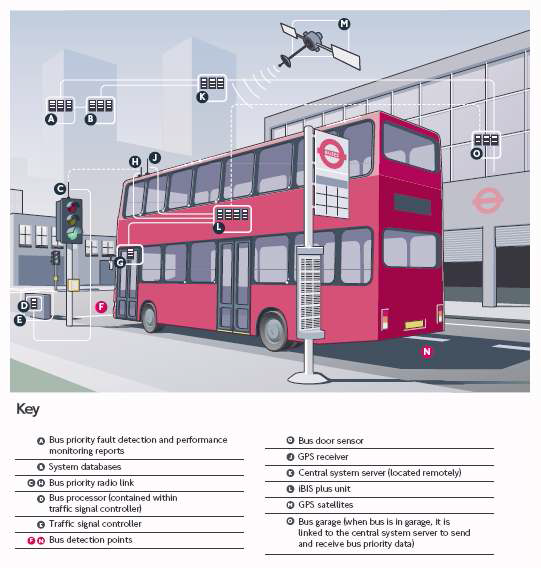
\includegraphics[width=1\textwidth]{Figures/iBus.png}}
	\caption{Overview of iBus System \cite{Hounsell201276}}
	\label{fig:iBusOverview}
\end{figure}
The OBU is responsible for a number of tasks including a regular (approximately every 30 seconds) transmission of the bus location. This information is currently used by the different bus operators for fleet management, as well as by CentreComm for real-time monitoring of the buses and their locations. There have been a number of other applications and systems that have been implemented and put in to use as a result of the data that is generated by the iBus AVL. Some examples include Countdown (real-time passenger information), improved bus priority at traffic signals and more \cite{Hounsell201276}. This has led to improved and more affordable transport service.

CentreComm operators have access to an online GIS system showing each bus location in the network on a map in real time. This system also allows them to see whether a given bus is behind, ahead or on time according to its schedule. However, this does not show or alert the control room staff if a bus or a route is disrupted. Control room staff can also see when was a given bus expected to arrive at a given bus stop and when it actually arrived. Again, this is only per individual bus and there are no automatic alerts set, in case a given route or stop is experiencing delays. Currently the work-flow is such that on-duty CentreComm staff needs to go and analyse all this information manually (once bus drivers or bus company operator have contacted/alerted the control room) in order to figure out if there is a problem and how severe it actually is. This is a very inefficient, tedious and error-prone process. Here is where this project comes into place to address the lack of preprocessed information and automated alerts.

\section{Related Work}
The literature is full of research towards accurately predicting bus arrival times with various computational models being used \cite{altinkaya2013urban}. Predicting bus arrival is complex as many factors need to be considered such as, bus dwell time at stops, general congestion and others \cite{jeong2005prediction}. This is also closely related to the issues of bus prioritisations for which we can find numerous examples in the literature. Some examples of work done towards bus prioritisation at traffic signals and junctions can be found in \cite{eps52676} and \cite{clarke2007}. However, these are not directly related to our problem domain and thus are not discussed further in this report. This is because we are not interested to know when is the next bus due to arrive at a stop or should we give priority to a bus at traffic signal. We want to know if buses experience increased travel time, because of which they get delayed travelling through some parts of the network. 
 
%The literature is abundant of research on addressing the issues of bus prioritisation at traffic signals and junctions \cite{eps52676} and \cite{clarke2007}, but this is not directly related to our problem domain and thus is not discussed further in this report.
 
%This however is not what this project is about as we are not interested to know when is the next bus due to arrive at stop, but we want to know if buses get delayed travelling through some parts of the network. 

The main problem posed by this project of detecting disruptions in the bus network can be also translated to short term traffic congestion detection and/or travel time calculation. This is valid as we are not interested in individual bus delays. Some examples of such single instances of bus disruptions are: customer incident on board of a single bus, technical fault with this bus or other issue(s) which are affecting a single vehicle rather than the entire route or network. We are interested into finding routes/sections in the network which are delayed/disrupted and this is beyond the control of individual bus operators. Most often such problems are due to some sort of congestion or road closures/repairs. However, road problems are in most cases linked with increased traffic congestions as roads are used by other vehicles as well. In order to address this problem we have focussed our attention towards work which relates to calculating the bus travel times or gives short-term traffic congestion predictions in a given transport network.

The literature contains plenty of work done toward detecting and calculating travel times in non-urban environment. This includes approaches based on AVL probe data and automatic vehicle identification (AVI), as well as induction loops \cite{Vlahogianni20143}. There is also plenty of research done towards traffic congestion detection based on AVL probe data \cite{Vlahogianni20143}. However, there are significant challenges due to the nature of the urban environment itself. Densely populated areas are influenced by many factors which can be affecting the general traffic flow. Another problem posed by urban environments is the irregularity of the AVL data transmission because of, for example weak or lost signal at times (e.g. due to high buildings) or even the presence of some noise which reduces the accuracy of the transmitted location. 

There is however, little research to my knowledge, which focusses on the issues of detecting and short-term forecasting traffic congestion/disruptions in arterial urban environment  \cite{Vlahogianni20143} \cite{5625144}. From the tables shown in figures ~\ref{fig:Vlahogianni201431} to ~\ref{fig:Vlahogianni201434} in Appendix A taken from \cite{Vlahogianni20143} we can easily see that most of what has been done has focussed on motorways and also has employed data from static detector points (e.g automatic vehicle identification). Only in recent years we can see that more attention has been given to the use of GPS and AVL data. This is probably due to increased popularity and usage of these technologies.

%As it can be seen from the tables in figures ~\ref{fig:Vlahogianni201431} to ~\ref{fig:Vlahogianni201434} shown in Appendix A taken from \cite{Vlahogianni20143}.

%For this reason in order to address our problem domain however we are not interested specifically in the general congestion as this could for example not affect the operation of the TFL bus fleet directly. A simple reason for this could be because there are significant amount of street which have a designated bus lanes which are prohibited for use by the general traffic. However there are studies showing that even under such circumstances there is a correlation between the general traffic flow and the performance of the buses in the same network [REFERENCE]. For our project we are interested however only in detecting the disrupted routes (sections of routes) and the severity of the disruption in the TFL bus network. We are interested in monitoring and detecting delays that are occurring in the network which would be classified, beyond the control of individual bus operator, by CentreComm.

%The literature review that has been undertaken as part of this project has showed that there are multiple approaches that could be undertaken to solve the problem posed by this project. There could be found different classifications of the models for predicting bus travel time\cite{surveyAIApplications}. According to \cite{urbanBusArrivalTimeCompModels} we could classify them into four computational models:
%\begin{itemize}
%	\item Based on historical data
%	\item Statistical 
%	\item Kalman Filtering 
%	\item Machine Learning
%\end{itemize}
%We could also add hybrid model which takes a combinational from the above [REFERENCE].

%The approaches and research that we have examined show us that the the main types of models that have been used for traffic forecasting according to \cite{youKim} can be categorised as follows:
In the literature various approaches to measure and predict travel time can be found. These models are categorised in four type groups according to \cite{youKim} as follows:
\begin{itemize}
	\item Statistical models - this type of models employ statistical tools and methods for analysis and forecasting. Some models of this type include:
	\begin{itemize}
		\item Historical
		\item Time Series
		\item Nonparametric regression
		\item Hybrid
	\end{itemize}
	
	\item Computer Simulations - main models of this type are traffic simulations. They allow simulation of the traffic flow in a network resembling the characteristic of moving vehicles. Main advantage of these models is that they allow for the simulation of different scenarios. The main drawback however, is that they require traffic flow prediction information in advance \cite{smith1997traffic}. Due to the optimisation nature of these approaches, usually high performance computers are employed (i.e. in \cite{junchaya1992advanced} they make use of parallel computing).
	
	\item Mathematical Optimisation - this include dynamic traffic assignment (DTA) models. A good review of dynamic traffic assignment and simulation models can be found in \cite{mahmassani1991review}.

	\item Artificial Intelligence (AI) - neural networks are an example of AI approach. They have received a lot of attention in terms of transportation systems applications. Some examples include traffic signal control, traffic flow modelling and transportation planning \cite{gilmore1995neural,Dougherty199721,smith1997traffic}.
\end{itemize}
The advantages and disadvantages of the listed types and models are summarised in table showed in figure~\ref{fig:modelsProsCons} below.

\begin{figure}[ht]
	\makebox[\textwidth][c]{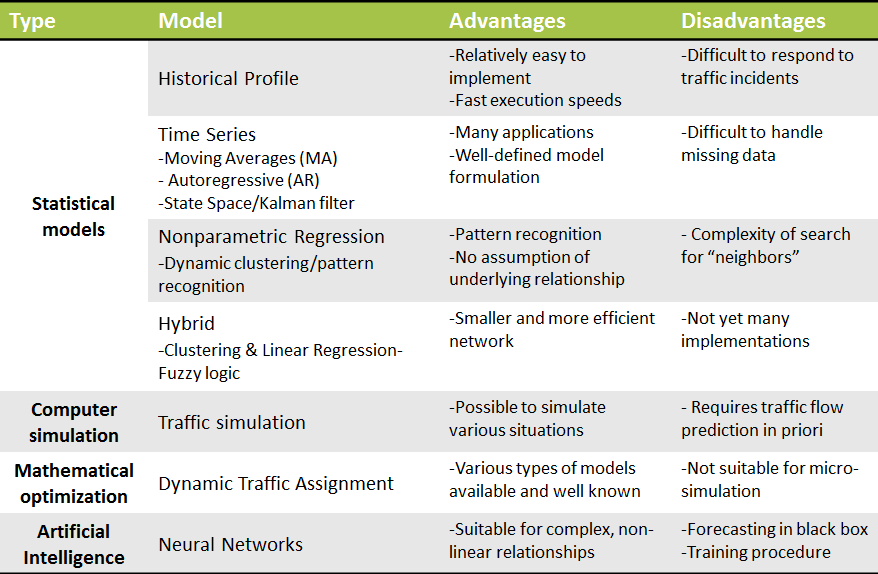
\includegraphics[width=1\textwidth]{Figures/modelsProsCons.png}}
	\caption{Traffic forecasting types and models \cite{youKim}}
	\label{fig:modelsProsCons}
\end{figure}

From the above mentioned, the most widely used and well defined are the statistical models. From them the historical approaches are relatively easy for implementation and have fast execution speed, but have difficulty with dealing with incidents. Time series models have many applications and are well formulated. Because of these reasons and also the nature of the data that has been made available (detailed description of which can be found in Chapter 5) for this project, we will focus our attention on time series analysis for the rest of this report.

\section{Time Series}
Time series is a sequence of data readings taken during successive time intervals \cite{shumway2010time}. This could be a continuous recording of readings or a set of discrete readings. In the context of our project we have the continuous process of bus readings (generated by the AVL system) being transmitted which generate a discrete set of observations. This results in a data set of measurement values which consists of the actual values with some noise. Time series data contains four main components (illustrated in figure~\ref{fig:timeSeriesDataComponents})\cite{brockwell2002introduction}:
\begin{itemize}
	\item \textbf{Trend} - this is the long term pattern that the given time series data follows. The trend can have positive or negative value depending on whether the data exhibits an increase or decrease respectively in the long term pattern. Time series data with no trend (it does not show nether increase or decrease) is said to be stationary.
	\item \textbf{Cyclical} - this is when we can see that the data show up and down movement around a given trend is referred to as cyclical pattern. Main characteristic of the cycle is its duration which can depend on the type of measurement.
	\item \textbf{Seasonal} - seasonality occurs when the time series exhibits regular repetetive fluctuations. For instance, temperatures peaks during summer months (in the northern hemisphere) and drop during winter months.
	\item \textbf{Irregular} - also known as the error component. These are random increases or decreases for a specific time period.
\end{itemize}

\begin{figure}[ht]
	\makebox[\textwidth][c]{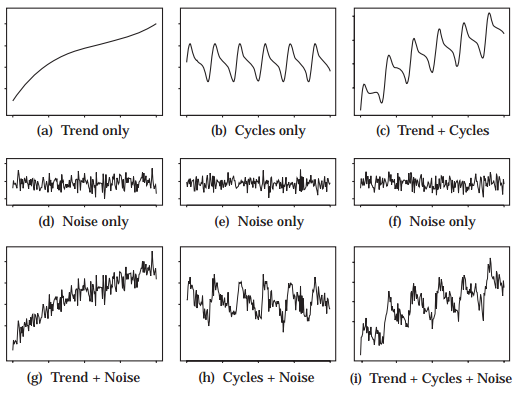
\includegraphics[width=1\textwidth]{Figures/timeSeriesDataComponents.png}}
	\caption{Time series data components examples taken from \cite{wildchance}}%taken from https://www.stat.auckland.ac.nz/~wild/ChanceEnc/Ch14.pdf
	\label{fig:timeSeriesDataComponents}
\end{figure}

Analysis of time series data could be performed in order to extract and calculate some meaningful statistics from the data \cite{shumway2010time}. This could also result in producing a forecast of the data of interest for the next (future/unobserved) period of time based on the past observations. In order to highlight trends and make predictions, we need to employ time series analysis techniques. Below I have presented some of the available techniques that could be employed when analysing time series data. This however, is not an exhaustive review of all available methods and models as I have tried to keep the discussion relevant to this project.

%Time series analysis is performed on time series data in order to extract some meaningful statistics from the data. In addition to the time series analysis time series forecasting could also be performed to come up with a prediction for the next period in time based on what has been observed in the past. In our problem this would mean having a number of bus readings we could analyse them and come up with prediction of what would be state in the next point in time. There also different smoothing techniques which would remove random abnormal fluctuation (e.g. an incident with a single bus).In the below sections we look at a number of different approaches to analysing and forecasting the next state of the network from the available data in real-time (we update our forecast whenever more data becomes available).

\subsection{Moving Averages}
One technique commonly used in time series analysis is moving averages which represent a form of smoothing. Smoothing means to dampen the effect of noise and irregularities in the original time series. Moving average, also called rolling or running average is a statistical calculation method. It helps to analyse data series by calculating a series of averages of subsets of the data. Moving averages are commonly used in time series data analysis when the data is fairly stable and does not have significant trend, cyclical or seasonal effects. It can be used in order to smooth out a time series data with the aim of highlighting or estimating the underlying trend of the data. The other main usage is as a forecasting method, again for time series. The main strength of these methods is that they are easy to understand. Moving averages are often used as the building block for more complex time series analysis. Below we present some of the main types of moving averages that are used in practice. \cite{brockwell2009time,shumway2010time}

%It is universal analysis technique. It is type of mathematical convolution \cite{shumway2010time}.It can also be referred to as rolling or moving mean and it acts like a filter.
\subsubsection{Simple Moving Average}
Simple moving average (SMA) is calculated by adding all the observations for a given period of time and dividing this sum by the number of observations. This is popular statistical technique which is mainly used to calculate the trend direction. The simple average is only useful for estimating the next forecast when the data does not contain any trends. Each observation is weighted equally. If we consider shorter period window (meaning we only consider less observation e.g. only the last 5 or 10) for our averages they would react quicker to changes. While if we work with bigger period windows the averages would have greater lag. The equation for calculating SMA is given below in equation~\ref{sma}. In this $n$ is the size of the window (e.g. the number of reading we are considering) and $Value(i)$ is the actual value of observation $i$. 

\begin{equation}\label{sma}
	SMA = \frac{\sum_{0\le i\le n}\textrm{Value(i)}}{n}
\end{equation}

In the table on figure~\ref{fig:smaTable} we can see sample time series data with window size $n$ equal to $3$. The graph in figure~\ref{fig:smaGraph} shows the plotted actual observation values and the SMA calculated predictions.

\begin{figure}[ht]
	\makebox[\textwidth][c]{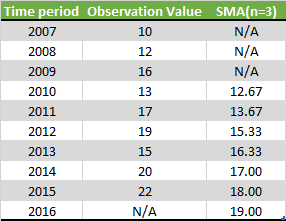
\includegraphics[]{Figures/smaTable.png}}
	\caption{}
	\label{fig:smaTable}
\end{figure}

\begin{figure}[ht]
	\makebox[\textwidth][c]{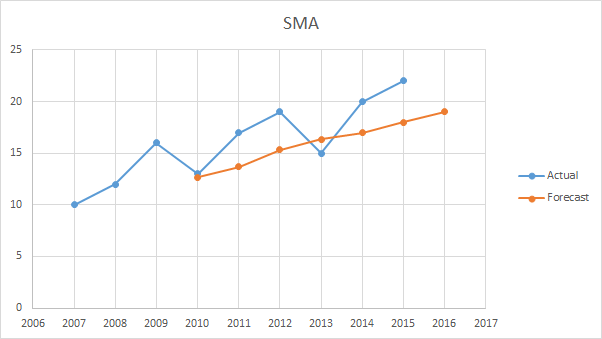
\includegraphics[]{Figures/smaGraph.png}}
	\caption{}
	\label{fig:smaGraph}
\end{figure}

Another form of SMA is centered moving average (CMA). Both are very similiar in terms that they use the same method for calculating the average value, but they differ in that the CMA calculates an average of $n$ periods' data and associates it with the midpoint of the periods. An example can be seen in figures~\ref{fig:cmaTable} and \ref{fig:cmaGraph}.

\begin{figure}[ht]
	\makebox[\textwidth][c]{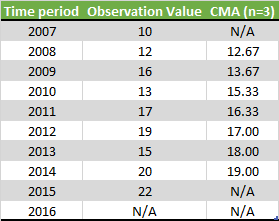
\includegraphics[]{Figures/cmaTable.png}}
	\caption{}
	\label{fig:cmaTable}
\end{figure}

\begin{figure}[ht]
	\makebox[\textwidth][c]{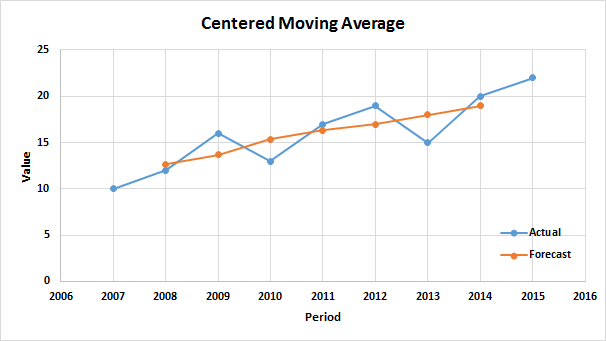
\includegraphics[]{Figures/cmaGraph.png}}
	\caption{}
	\label{fig:cmaGraph}
\end{figure}

\FloatBarrier
\subsubsection{Weighted Moving Average}
The problem with the simple moving average is that it weighs all data points equally, meaning that both older and newer data would have the same effect on the average. This however, is not the case when using weighted moving average (WMA). In WMA model each data point would be weighted differently according to the period of time when the observation was made. For example, if we consider a $n$ period moving average we can calculate the weight for the value taken in period $i$ where $0\le i\le n$ by the following formula: \[\textrm{Weight(i)} = \frac{2i}{n(n+1)}\] This would mean that recent data has bigger impact on the result. However it should be noted that the weighting formula given is only an example as it is the most natural and widely used weigthing scheme for WMA. It is possible to use different weighting formula, one such alternative could be: \[\textrm{Weight(i)} = \frac{2^i}{\sum_{0\le x\le n}2^x}\] this would result in putting more weight on more recent data (e.g. older data is having less effect). The general equation for calculating WMA is given below as equation~\ref{wma}, where $n$ is the number of observations (the size of the window).

\begin{equation}\label{wma}
WMA = \frac{\sum_{0\le i\le n}(\textrm{Weight(i)}\textrm{Value(i)})}{\sum_{0\le i\le n}Weight(i)}
\end{equation}

An example of the application of WMA is shown in the table in figure~\ref{fig:wmaTable}. The forecast is plotted against the actual values and is shown in the graph in figure~\ref{fig:wmaGraph}

\begin{figure}[ht]
	\makebox[\textwidth][c]{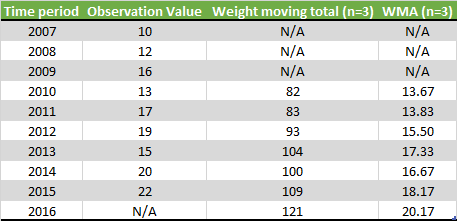
\includegraphics[]{Figures/wmaTable.png}}
	\caption{}
	\label{fig:wmaTable}
\end{figure}

\begin{figure}[ht]
	\makebox[\textwidth][c]{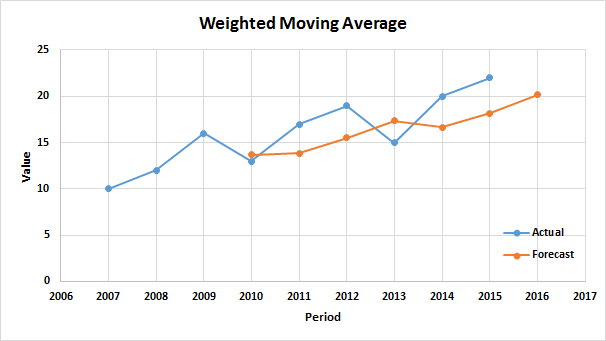
\includegraphics[]{Figures/wmaGraph.png}}
	\caption{}
	\label{fig:wmaGraph}
\end{figure}

\FloatBarrier
\subsubsection{Exponentially Weighted Moving Average}
Exponential smoothing was first suggested by Robert Goodell Brown \cite{FOR3980040103}. Exponentially weighted moving average (EWMA) or also called exponential smoothing or simply exponential moving average (EMA) is very similar to WMA. The main difference is that in order to calculate it, we do not need to keep all the data, but we could only store the latest value and the previous forecast only. Exponential moving average weights the data points exponentially which means that the oldest data would have minimalistic effect on the result. There exist a few exponential smoothing techniques including single, double and triple exponential moving average [REFERENCE]. Equations 2.3 and 2.4 give the simplest way for calculating single exponential smoothing. In this equation $\alpha$ is called the smoothing factor and it is usually a value between $0$ and $1$. The closer $\alpha$ is to $0$, the greater smoothing effect it has. This however makes it less responsive to recent changes thus produces greater lag. Values of $\alpha$ that are near to $1$ have less smoothing effect, but are very reactive to recent changes in the data. 

\begin{align}\label{ema}
EMA_1 = Value_1 \\
\textrm{for } t > 1\textrm{, }EMA_t = \alpha Value_t + (1-\alpha) EMA_{t-1}
\end{align}

Example of the application of EMA with different values of $\alpha$ ($0.2$ and $0.8$) is shown in figures~\ref{fig:emaTable} and~\ref{fig:emaGraph}. From this simple example it can be clearly seen the effect the value of $\alpha$ has on the output value. From the graph (figure~\ref{fig:emaGraph}) it can be seen that the smaller $\alpha$ value of $0.2$ has greater smoothing effect, but greater lag. The bigger value of this constant increases the reactivity to recent changes, but produces less smoothed line.
\begin{figure}[ht]
	\makebox[\textwidth][c]{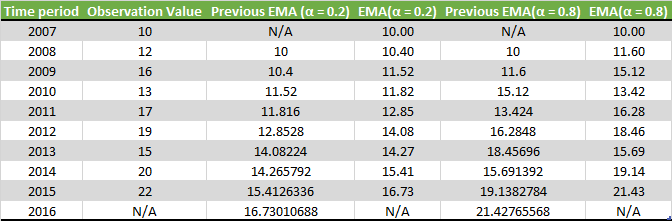
\includegraphics[]{Figures/emaTable.png}}
	\caption{}
	\label{fig:emaTable}
\end{figure}

\begin{figure}[ht]
	\makebox[\textwidth][c]{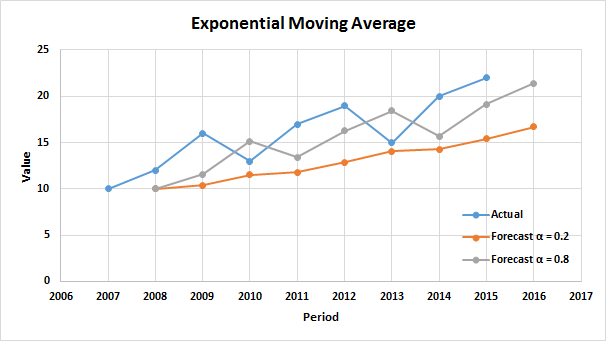
\includegraphics[]{Figures/emaGraph.png}}
	\caption{}
	\label{fig:emaGraph}
\end{figure}
%Exponential Smoothing for Predicting Demand. Cambridge, Massachusetts: Arthur D. Little Inc. p. 15.] and then expanded by Charles C. Holt in 1957.[Holt, Charles C. (1957). "Forecasting Trends and Seasonal by Exponentially Weighted Averages". Office of Naval Research Memorandum 52. reprinted in Holt, Charles C. (January–March 2004). "Forecasting Trends and Seasonal by Exponentially Weighted Averages". International Journal of Forecasting 20 (1): 5–10. doi:10.1016]
\FloatBarrier
\subsubsection{Summary}
If we compare the presented moving average methods (SMA, CMA, WMA and EMA) we can clearly see that the SMA and CMA offer the most smoothing. However, this comes with the trade-off of an increased lag (e.g. it takes longer to reflect recent changes). 

The weighted moving average performance is influenced by the choice of window size, as well as the choice of weights. There is no single rule what weights one should use and most often this is based on intuition and simulations in order to get optimal results.

As we have seen in the given examples, the exponential moving average performance depends heavily on the chosen values for the $\alpha$ constant. EMA offers the advantage of not having to keep all data point values in memory for the periods of our window. Whereas all the other presented techniques require us to specify a widow size for our moving average and also to have the data for these periods available in memory. The choice of window size for the SMA, CMA and WMA has direct impact on the sensitivity (speed of reaction) of the method to changes. Increased size of the window results in less reactive moving average and increase in the opposite.

If a trend indication with better smoothing and little reaction for shorter movements is required, then the simple average should produce the best results. However if smoothing is desired where you can still see shorter movements, then it is better to use either WMA or EMA. Using either of those techniques, requires us to make some choices regarding what parameters (window size and weight for WMA and value of $\alpha$ for EMA) to use in order to obtain best results.

%will react faster to changes and sits closer to the actual readings, however it might overreach at times. 
%The weighted moving follows the movement even more closely than the exponential moving average. Determining which one to use depends on the objective. 

\subsection{Peak Detection}
Peaks and valleys represent significant events where the graph changes from increasing to decreasing behaviour and vice versa (decreasing to increasing). In the domain of our project we are mostly concerned with peak detection as we are not interested to know if buses are gaining time (e.g. are going ahead of schedule). Mathematically viewed peaks and valleys represent local maxima and local minima respectively \cite{simon1994mathematics}.

Detection and analysis of peaks (spikes) and valleys in time series is important in many applications (e.g signal processing, bioinformatics, medicine and many more) \cite{ventzas2011peak}. Peaks and valleys usually represent either significant events or errors in time series data. In our domain we are mostly interested in detecting high sudden changes in the traffic congestion conditions (e.g along route/sections in the bus network). In figure~\ref{fig:peakExampleGraph} we can see an example of such peak (highlighted in red) we would be interested to detect.

\begin{figure}[ht]
	\makebox[\textwidth][c]{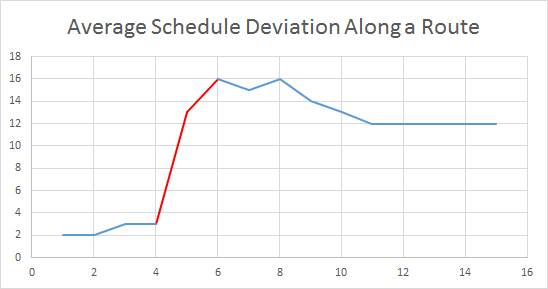
\includegraphics[]{Figures/peakExampleGraph.png}}
	\caption{X-axis shows us the sections along the route and the Y-axis represents the schedule deviation in minutes}
	\label{fig:peakExampleGraph}
\end{figure}

Peaks could be easily identified by visualising the data as in the above example. However, to be relevant and useful in real application this process should be automated. Various peak searching algorithms are studied and presented in \cite{ventzas2011peak}.

%In the literature has many examples of peak detection application one such for example is \cite{simplePeakDetection} used for spike detection in microarray data (anther example could be found in \cite{Azami2014491}).

%We do not go into details of any particular algorithms here because of the time constraints of this project (a study peak detection algorithms could be found in \cite{ventzas2011peak}).

\FloatBarrier
%\section{Other}
%However it is worth to note that spike detection and analysis could be used to classify events that are detected. A simple example could be to distinguish if given detected congestion/disruption is incident related (e.g. sudden) or it is general traffic jam (e.g. rush hour).
%[MOVE THIS TO CONCLUSION AS DIRECTION FOR FUTURE WOKR] - check this http://www.cs.technion.ac.il/users/wwwb/cgi-bin/tr-get.cgi/2012/CS/CS-2012-06.pdf
%Other approaches that could be used include Kalman filtering \cite{kalmanFiltering} \cite{Guo201450}, Markov Chains \cite{Qi201495} \cite{Ramezani20121576}, Machine learning \cite{herring2010real}, Bayesian networks \cite{Wang201479}. 

%In this report we do not go into further details of these alternative  as the aim of the project is to fully understand the requirements of the CentreComm and propose a prototype which to serve as a proof of concept.
%Markov chain is a stochastic process that transitions from one state to another using some state space. It is characterised by the property of having no memory. This means that the next state depends only on the current state and not on the preceding sequence of state transitions. This is called a Markov property.
%Markov chains are usually used in modelling many practical problems. They are also effective in modelling time series. In this paper, we apply the Markov chains model to analyse and predict the time series. Some series can be expressed by a first-order discrete-time Markov chain and others must be expressed by a higher order Markov chain model. Numerical examples are given. The results show that the performance and effectiveness of the Markov chain model to predict the time series is very well.[TAKEN FROM - Application of Markov Chains to Analyze and Predict the Time Series]

\section{Summary}
In this chapter I have aimed to provide the reader with broad view of the background of our problem and its domain. Detailed overview of the operations, technologies and work flows used by TFL's bus command and control centre has been provided. This has led to detailed review and discussion of the related work found in the literature. The chapter concluded with discussion on some of the available time series analysis methods that can be used in our project. The exact approach taken and any implementation specifics are described in detail in Chapter 5, along with presentation and discussion of the data that has been provided by TFL for this project.
\chapter{Specification}
In this chapter I have introduced and formalised the user and functional requirements.
This is an important step of any project, especially computer science project, as it formalises the problems that the project is trying to address as outlined by the project aims and objectives in Chapter 1. It also allows to be used as a measure for evaluating the success of the project once it has been completed. The requirements presented below have evolved and have been refined throughout the project lifetime in response to feedback from and discussions carried out with, the key stakeholders.

\section{User Requirements}
The user requirements provide a list of the functionalities that the user(s) expect(s) to be able to perform and see/obtain the according results, in the end product system. These are what is expected from the system, but are not concerned how they are designed or implemented. The main user requirements are listed as follows:

\begin{enumerate}
	\item The tool must be able to produce a prioritised list of the disruptions in
the bus network that it has knowledge of.
	\item The tool must be prioritising the disruptions according to the user defined
rules (these are still discussed and gathered from the user).
	\item The tool must be updating this list of disruptions whenever there is more
data. This should happen as real-time as possible.
	\item The tool must be able to provide detailed information for every detected disruption. This has to include the specific section and route that are affected and its severity.
	\item The user must be able to interact with the system in order to lower or
increase the priority of a given disruption (even ignore one).
\end{enumerate}

\section{Functional Requirements}
These requirements specify in more details what the expected behaviour and functionality of the system/tool is. They are built on top of the user requirements as an input and are detailed list of what the system should be able to accomplish technically. The tool/system must:

\begin{enumerate}
	\item Have an appropriate and useful representation of the bus network in order to be able to monitor and detect problems in it.
	\item Be able to read and process CSV files as this is the primary input of the AVL feed files (more detailed discussion on the exact input and its format is presented in Chapter 5).
	\item Listen/monitor for new incoming data and process it in as close as possible to real time.
	\item Be able to update itself whenever new data is detected and processed.
	\item Be able to run without intervention 24/7.
	\item Keep track of the disruptions detected and track how they evolve and develop.
	\item Be able to keep information for a given window of time (e.g. data feeds from the last 2 hours).
	\item Be able to output a prioritised list of disruptions.
	\item Visualise the generated output appropriately.
	\item The system should be compatible with and accessible from every CentreComm staff's computer. Extension of this requirement is that it should be accessible from other teams and groups inside TFL.
	% It should be compatible to run under Firefox or Internet Explorer as this are the main browsers used by CentreComm/TFL staff.
	\item Display on request detailed information for the respective disruption. This should include a graph representing the route/section average disruption time.
	\item Be easy to deploy, configurable and maintainable.
\end{enumerate}
\chapter{Design}
For the purpose of the successful completion of this project I have decided to employ agile software development methodologies with evolutionary prototyping. The reason for taking this approach are the strengths of the agile software developmental methodology which is that it is incremental, cooperative, flexible and adaptive \cite{4147390}. Our project is addressing an issue which does not have well specified set of requirements and the clients do not have a clear view of what they actually expect. This led us to use  evolutionary prototyping \cite{Connell89} as this helps minimise the impact of misunderstanding or miscommunication of the requirements. The risks of which are relatively high as the goals of this project are relatively new and there is very limited similar work done. This technique would also give better idea of what the end product would be capable of and would look like to the client. With evolutionary prototyping the system is continuously refined and improved. Each iteration builds on top of the previous, thus meaning that with each increment more functionality is added and features and/or refine/improve what has already been implemented. Simply stated, this means that with each increment the system moves one step closer to the end product. This allows us to add features which were not previously considered or remove ones that are no longer viable or needed. In addition, this approach allows us to engage with the key stakeholders very early in the project life-cycle. This will provide us with valuable feedback which again brings a lot of advantages:
\begin{itemize}
	\item The delivery of the tool is speeded up and also minimises the risks of failing to deliver a working product before the project deadline \cite{Connell89}.
	\item Users would engage with the product early in the project lifetime. This however, poses some risk like the users requesting more features which were not previously mentioned or discussed. This means that I need to maintain some balance as this project has a fixed deadline and limited resources.
	\item Increased chances of fully understanding and meeting the user's requirements and expectations from the tool.
\end{itemize}
Each increment (iteration) consists of the following stages:
\begin{enumerate}
	\item Requirements specification \& refinement
	\item Design
	\item Prototype implementation \& Testing
	\item User testing and feedback provision
	\item Evaluation
\end{enumerate}
The requirements and specification step would document what the tool should look and work like at the end of each iteration. These would be following the aims and objectives I have defined in Chapter 1 of this report. After a prototype has been implemented and tested by the user, I will evaluate the progress and make any changes in the requirements, design and project plan accordingly. Thus after a number of iterations, the developed prototype will (should) resemble the desired product as required by the user.

In the below sections I have presented the system at an abstract level. This follows from careful analysis and consideration of the requirements stated in the previous chapter. I have tried to highlight all major key components and classes which are described formally. This allows us to better organise and structure our problem. The diagrams presented follow the unified modelling language (UML) paradigm \cite{uml} and are platform-independent models (PIM) of the system. This allows us to focus on the design of the system itself without distracting our attention with platform specific decisions. Once these models are created they can then easily be transformed into platform specific models (PSM) using the desired technologies.
%we can than easily transform them into platform specific models (PSM) using the desired technologies.
%This technique is known as Model-Driven Architecture (MDA) software design approach \cite{mda}.

\section{Use cases}
Based on the user requirements stated in the previous chapter, a use case diagram has been derived and presented in figure~\ref{fig:useCase} below. The use case diagram depicts the way users (actors) interact with the tool (system). There are three types of users of the system (every next type is extension of the previous as it can be seen from the diagram):
\begin{itemize}
	\item \textbf{Normal} users are people with general access to the system. They have read-only right and can interact with the system by requesting a list of disruptions and more details for a selected from them disruption. They also have access to the disruption history of the network. This use case was not in the initial requirements and was identified as a useful feature during demonstrations of the prototype to TFL.
	\item \textbf{Operator} is assumed to be a CentreComm staff member who is required to authenticate into the system. This would allow them the extra functionalities of adding comments to disruptions for others to see. Such users also have the functionality of hiding and showing disruptions that are currently detected in the bus network available to them.
	\item \textbf{Administrator} users have the most privileges of all type of users of the system. In addition to the above actions they are also allowed to view and change the configuration settings of the system. This is to allow easier configuration of the application.
\end{itemize}

\begin{figure}
	\makebox[\textwidth][c]{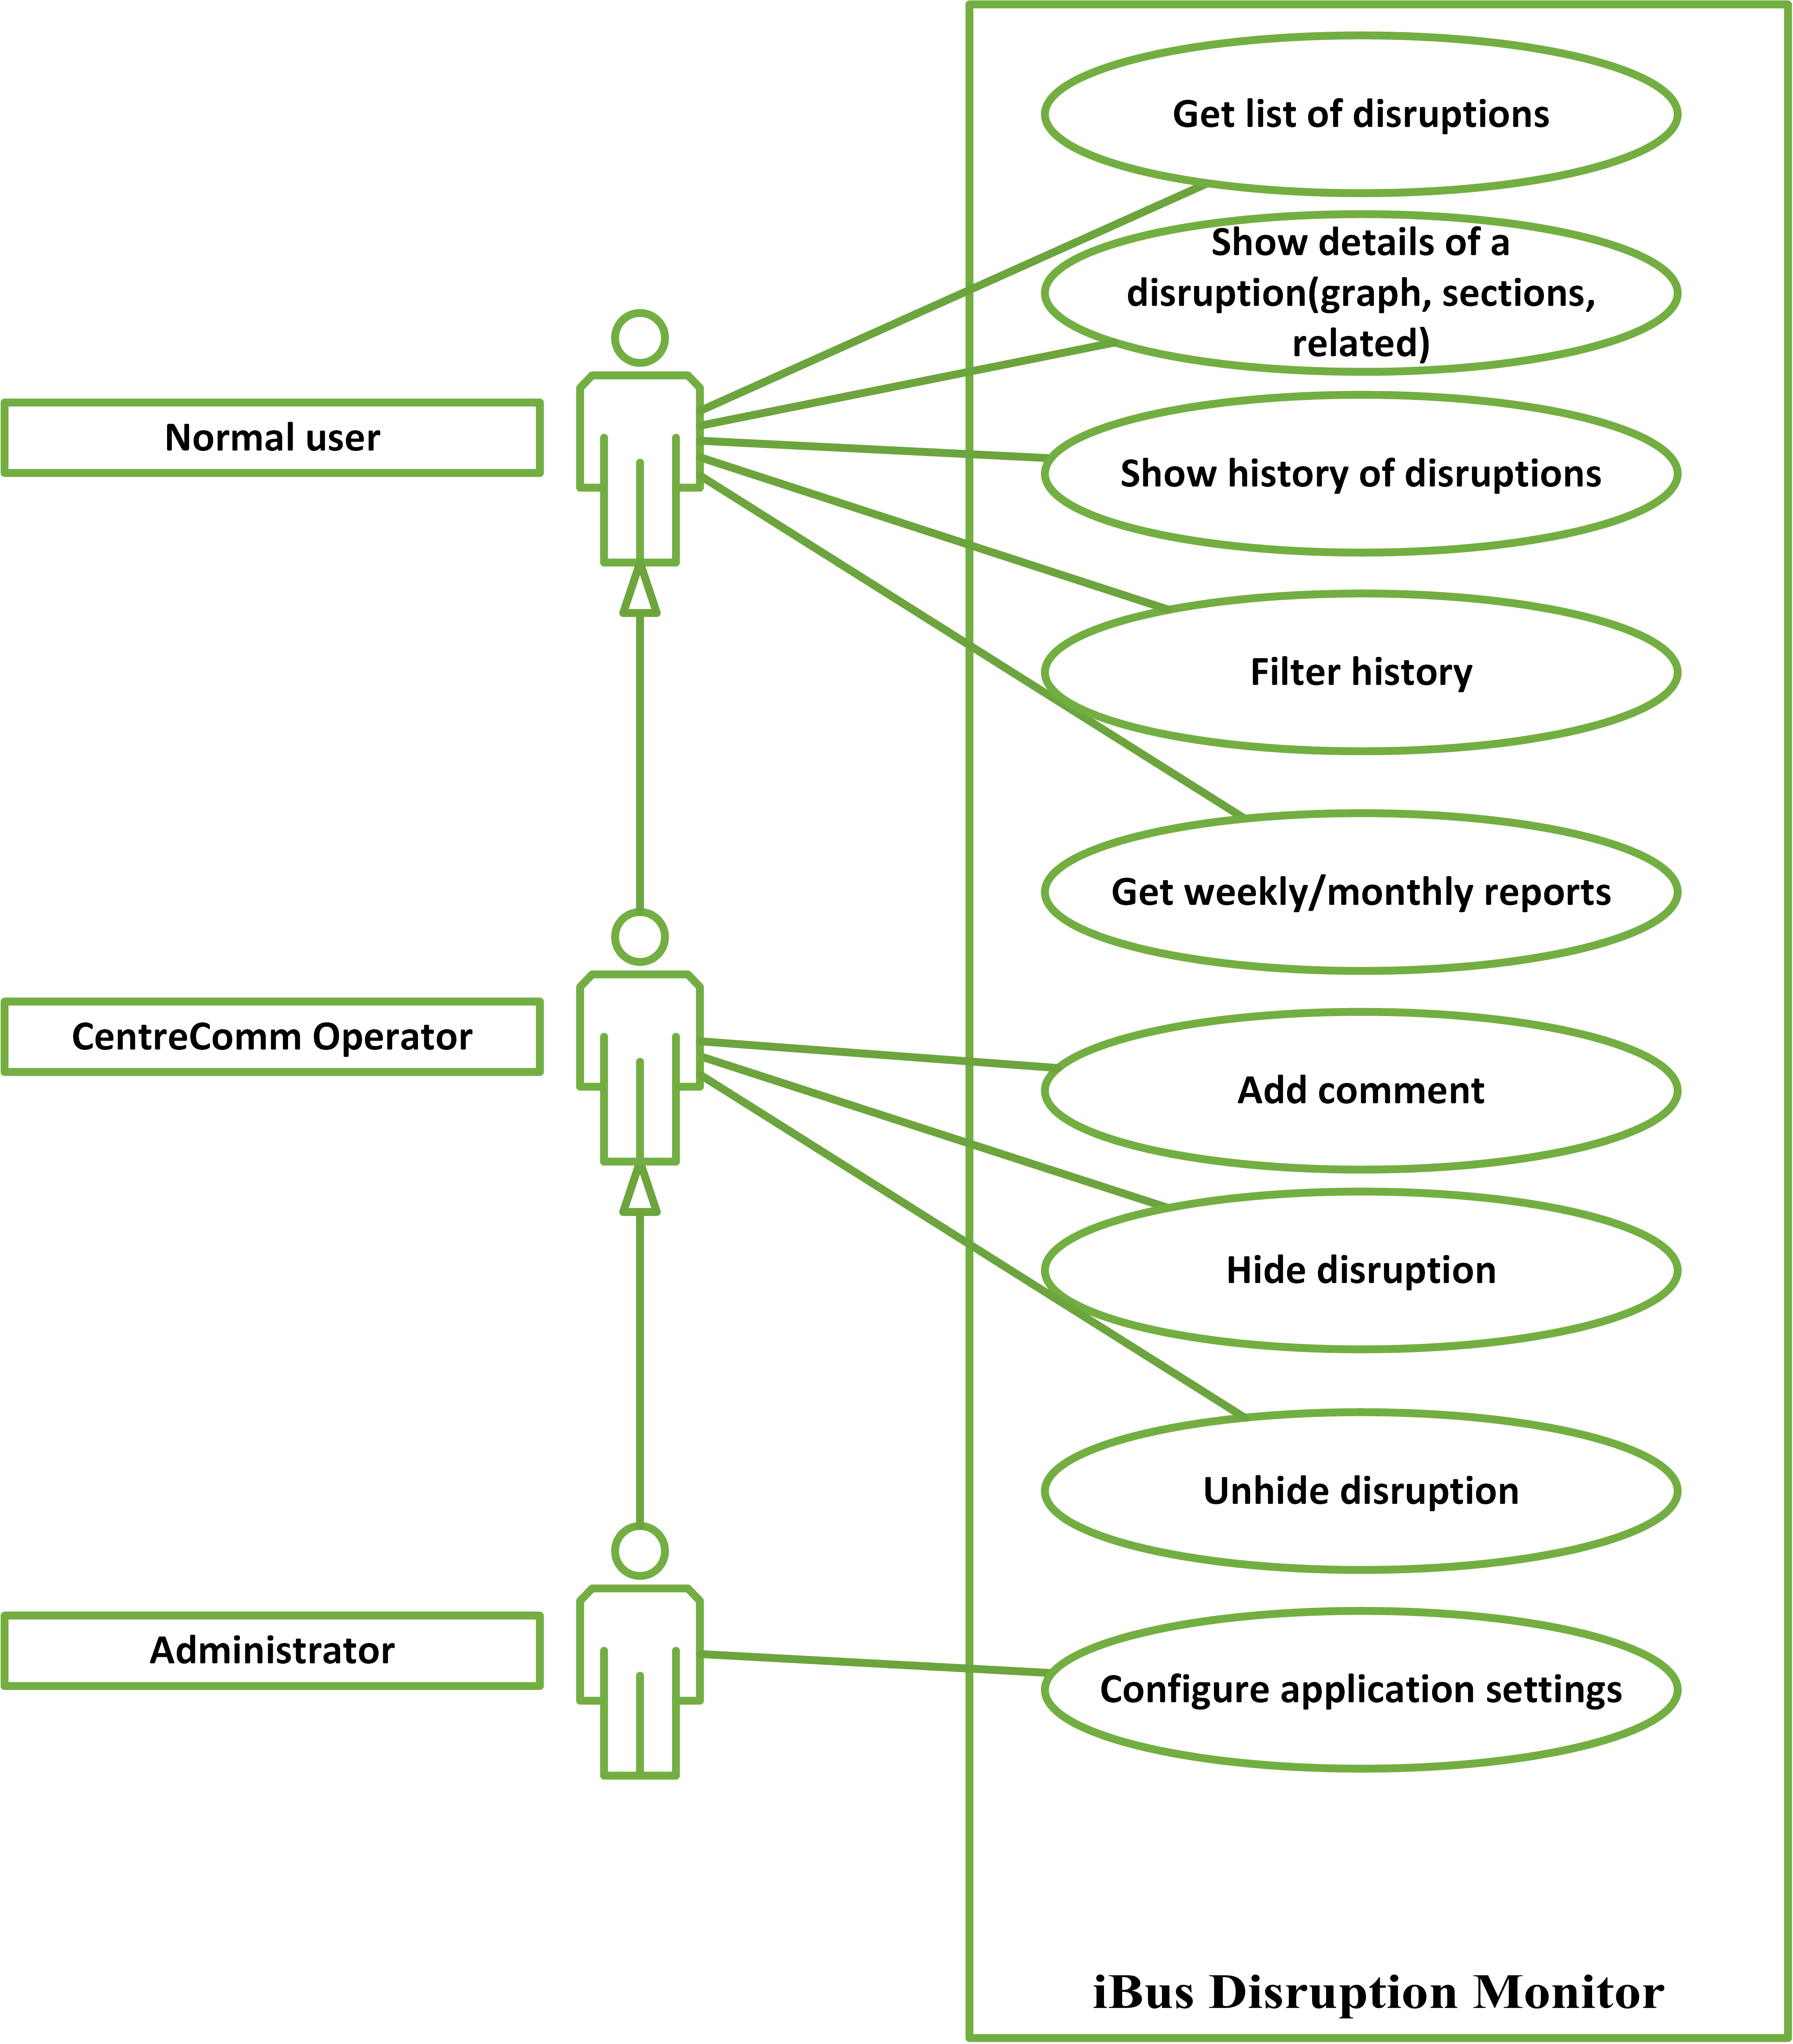
\includegraphics[width=1.2\textwidth]{Figures/UseCases.png}}
	\caption{Use Case Diagram}
\label{fig:useCase}
\end{figure}

\FloatBarrier
\section{System architecture}
In figure~\ref{fig:systemArchitecture} the architecture diagram of the system could be seen. The overall architecture is following a four-tier architecture with a model view controller (MVC) pattern for the user interface. This structure allows us to decompose to system into separate subsystems where lower tiers do not depend on higher tiers. This system allows for the implementation details of subsystems to be changed without affecting other components if the interfaces do not change.

As it can be seen from the diagram the system is divided in four main layers:
\begin{itemize}
	\item \textbf{Representation Layer} - It consists of a number of user views and is responsible for visualisation of the user interface. 
	\item \textbf{Representation  Control Layer} - responsible for the control/transition between user interface windows. In this layer I have made use of the front controller pattern \cite{fowler2003patterns} as it allows us to combine the common logic in one controller.
	\item \textbf{Application Logic Layer} -  this layer is the functional core of the system. This is where all the business logic is encoded and corresponding calculations are done. The most important part of the system is the Disruption Engine which is responsible for:
	\begin{enumerate}
		\item Monitoring for new feeds and processing them.
		\item Updating the bus network status (calculating delays and detecting disruptions).
		\item Writing the changes to the system database.
	\end{enumerate}
	The Disruption Model is the other major component of the system. It is responsible for retrieving the disruptions and their details from the database and providing them to the representation control tier.
	\item \textbf{Data Layer} - this is the data repository layer responsible for storing and maintaining the underlying system data. It consists of comma separated values (CSV) files representing the AVL feeds that are being pushed to the system. Here we also have the system database which contains all the configuration settings parameters and the output of the engine (disruptions and their details that are detected by the tool).
\end{itemize}
The architecture diagram shown in figure~\ref{fig:systemArchitecture} represents coarse grained view of the system to be implemented. Each of the components presented above could be implemented as a number of smaller components and modules depending on the specific technologies.

\begin{figure}
	\makebox[\textwidth][c]{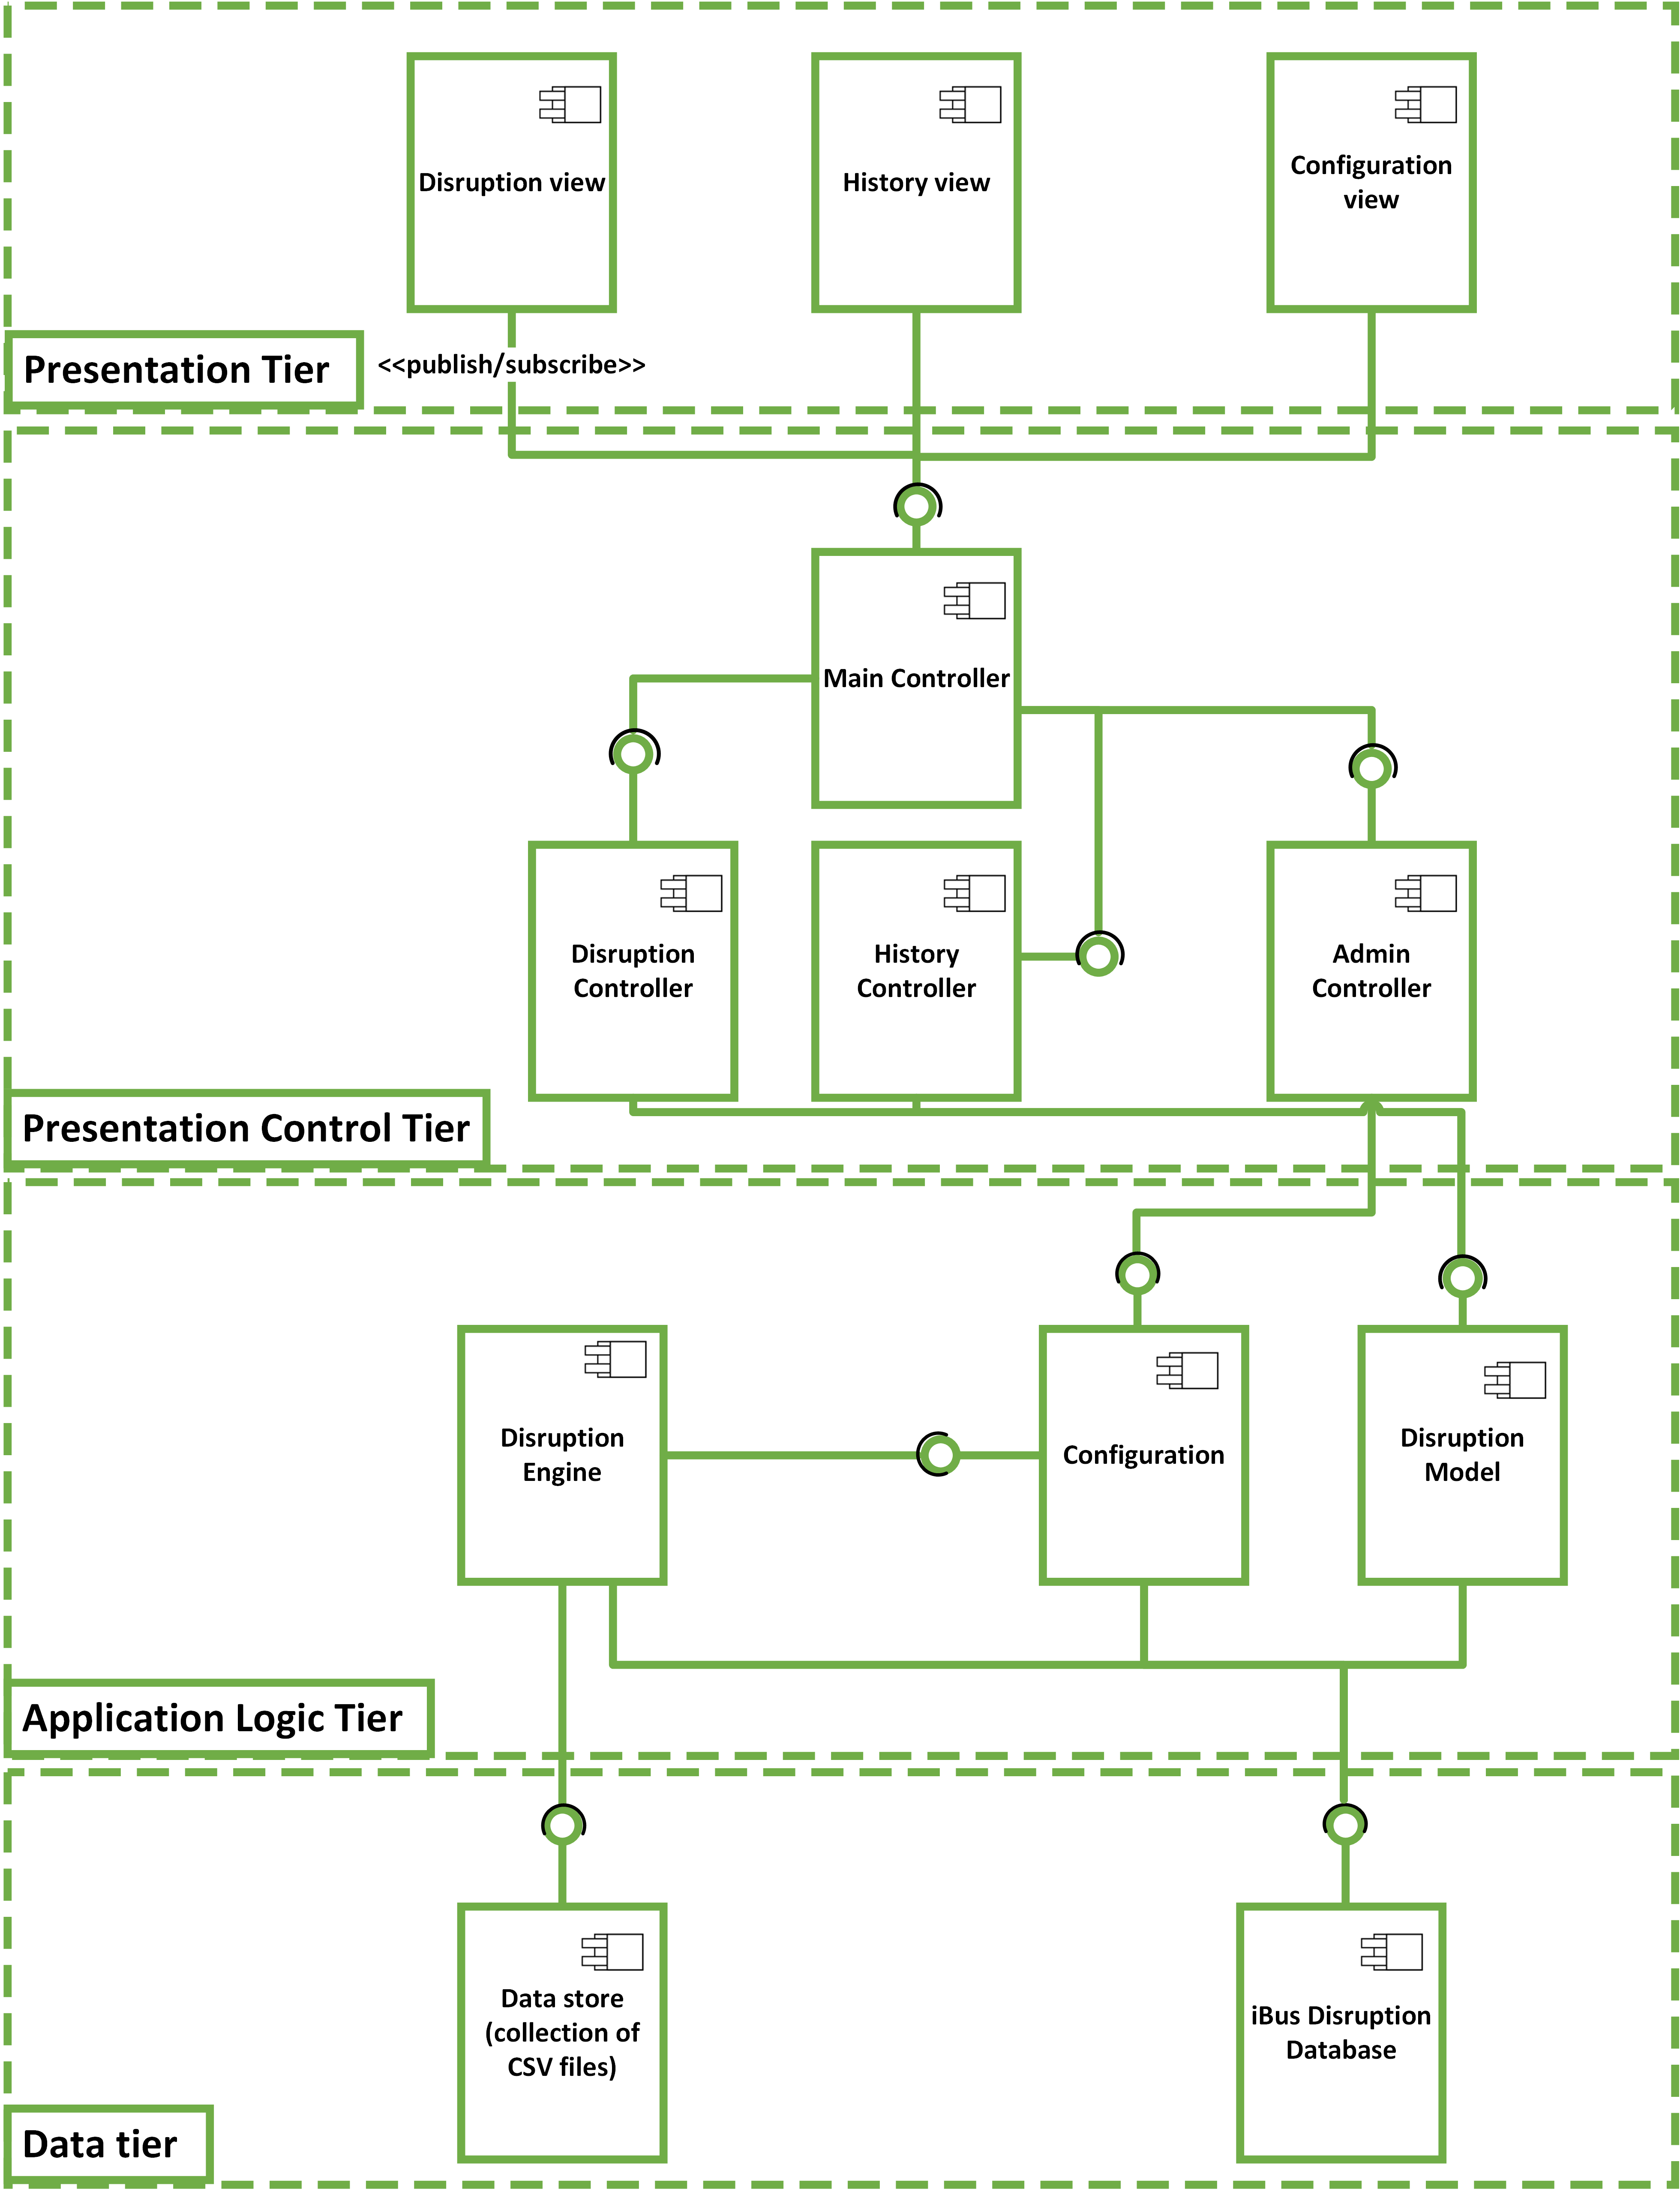
\includegraphics[width=1.2\textwidth]{Figures/Architecture.png}}
	\caption{System Architecture Diagram}
\label{fig:systemArchitecture}
\end{figure}

\FloatBarrier
\section{State Machine}
State machine diagrams are useful in explaining in what states the system could reside and how it transitions from one state to the other. The state machine diagram of the disruption engine component of our system is presented in figure~\ref{fig:stateMachine} below. This diagram represents the states in which the disruption engine could reside and the available transitions. As it can be seen from the figure, once the engine is initialised correctly it enters a continuous loop. This loop represents the engine waiting for new feeds to be detected by the system. Once detected they are processed and the bus network state is updated. If this update results in no changes in the state of the bus network compared to the previous observed state, the tool does not make any changes to the database, else it would write all the changes that have been detected and calculated. In case the system fails to connect or write the changes to the database the system terminates producing the appropriate error alerting the maintenance personnel. This behaviour is appropriate for this project as its scope is to produce a proof of concept working prototype rather than a fully functional ready to deploy production tool.

\begin{figure}
	\makebox[\textwidth][c]{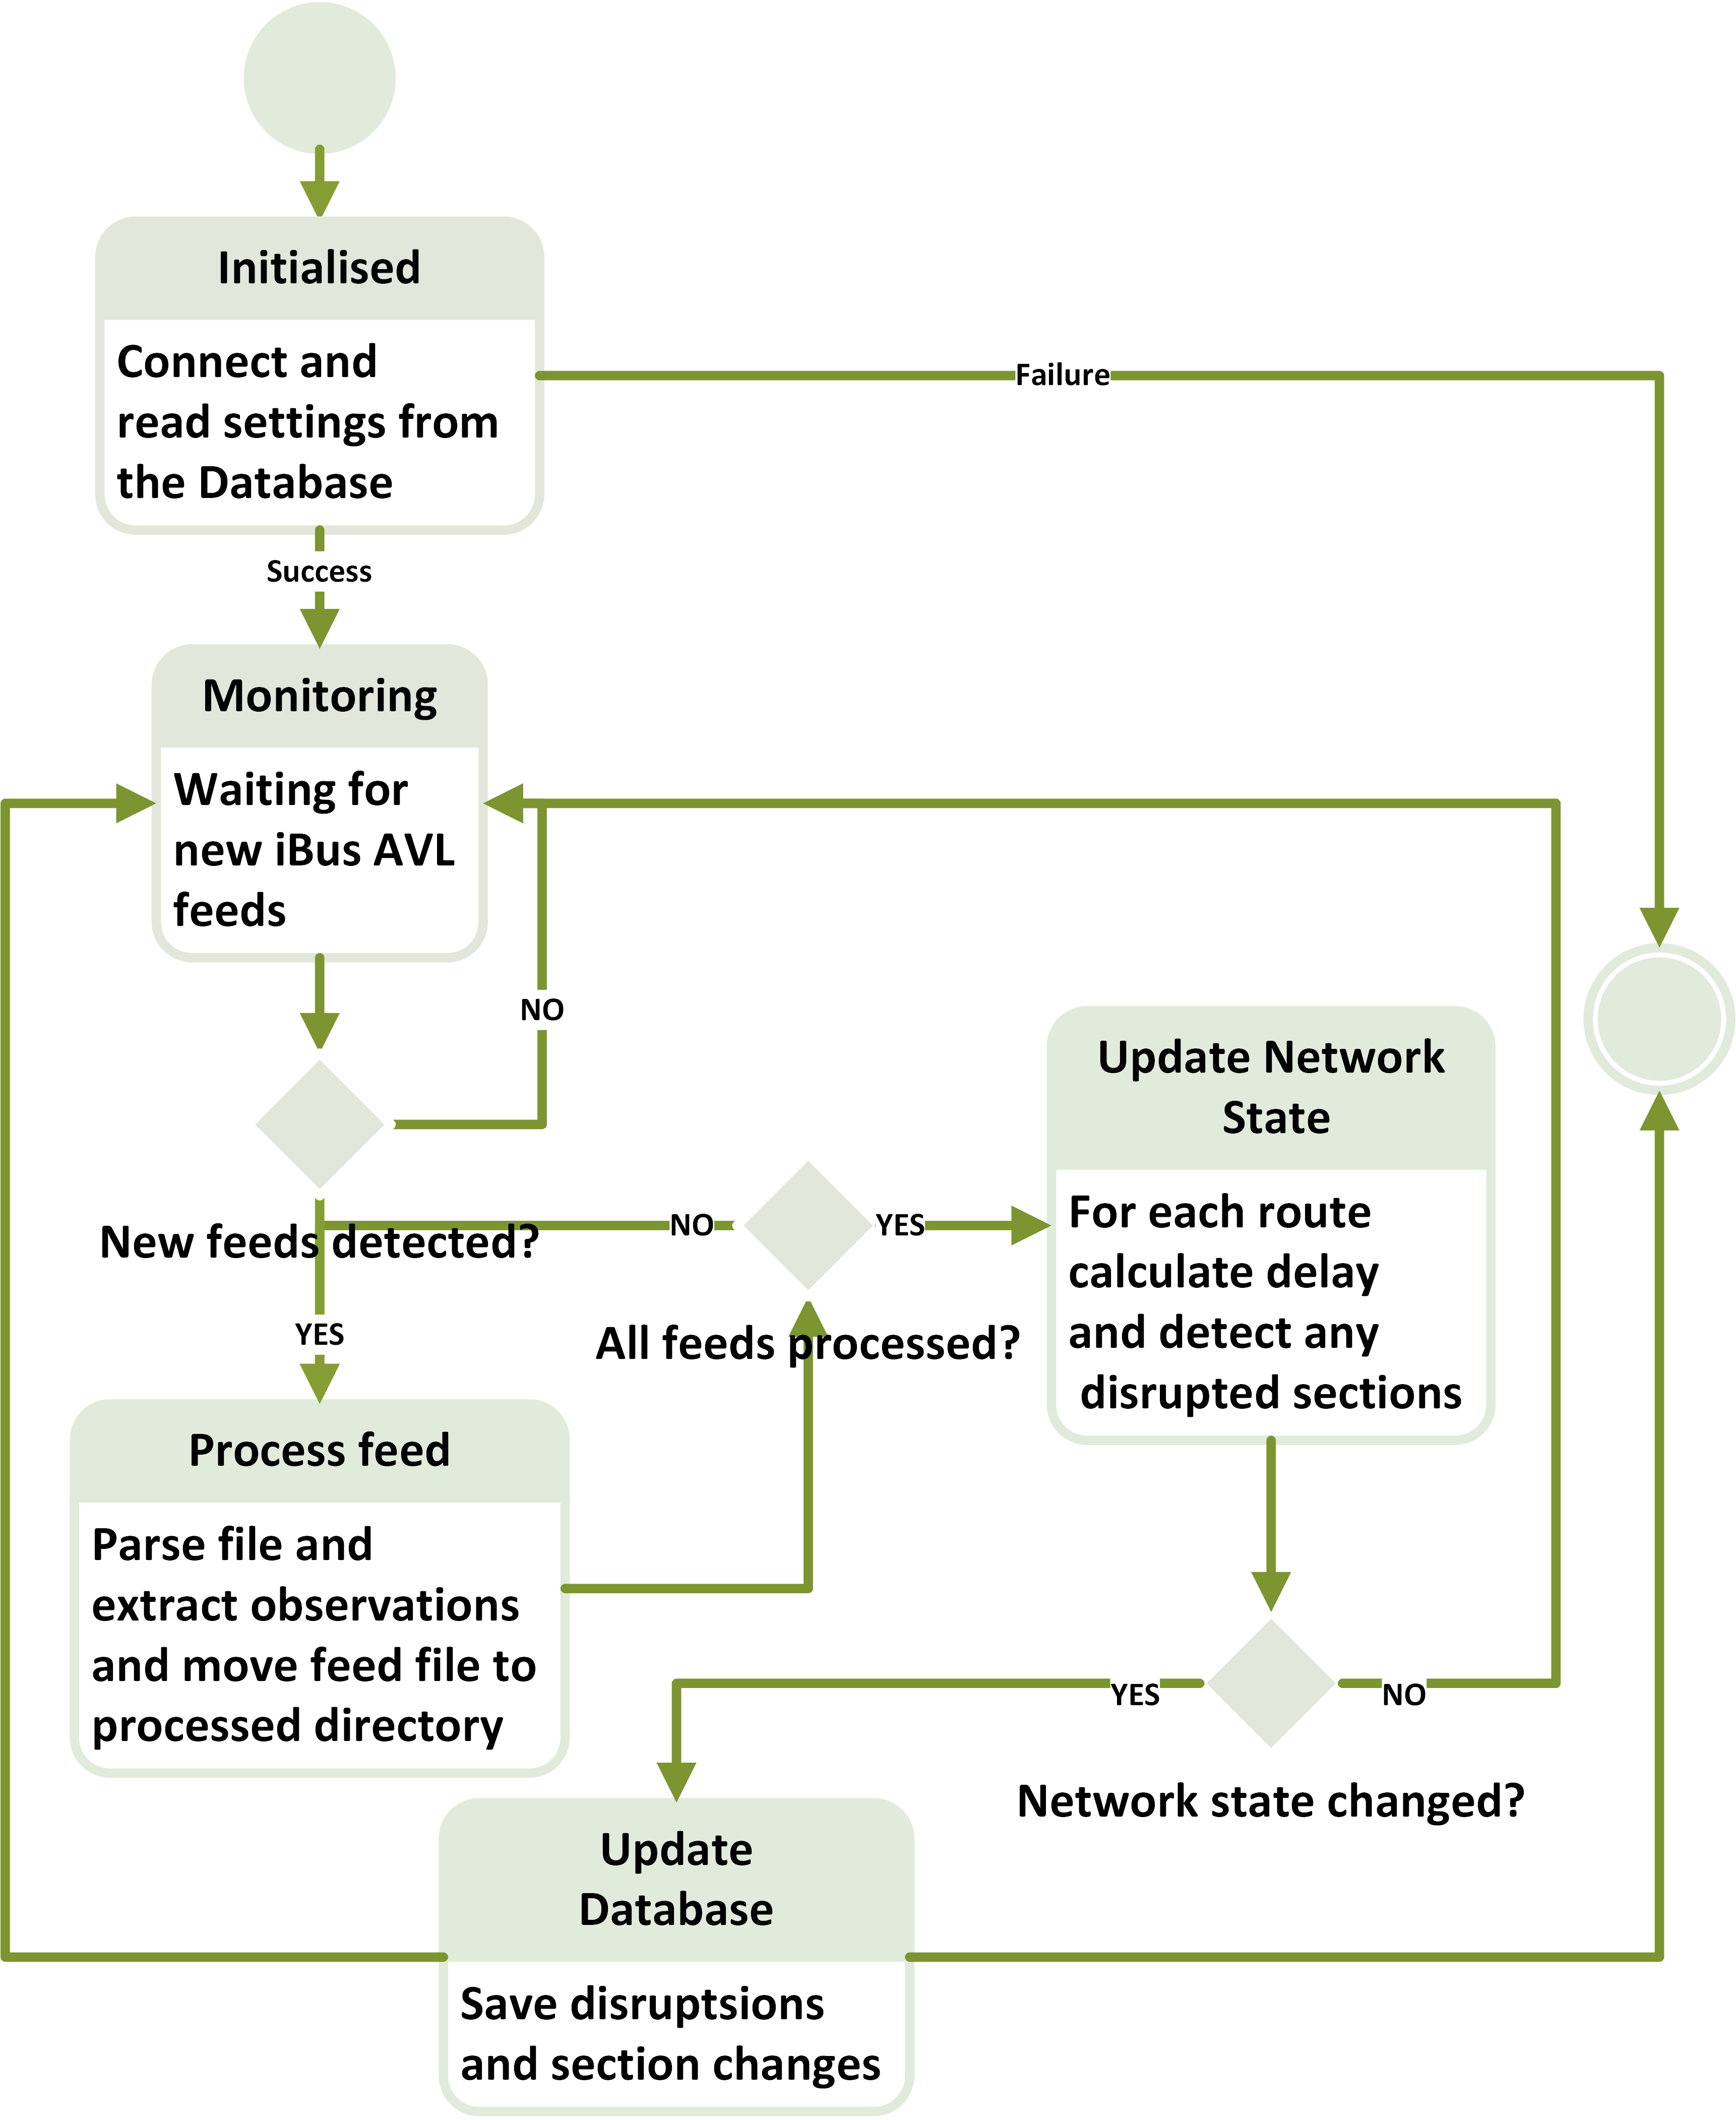
\includegraphics[width=1.2\textwidth]{Figures/StateDiagram.png}}
	\caption{State Machine Diagram}
\label{fig:stateMachine}
\end{figure}

\FloatBarrier
\section{Class organisation}
Class decomposition diagrams are the main building block of object oriented programming paradigm. They are a widely used tool for the organisation and design of a software system. The diagram consist of classes, which encapsulate some attributes (state) and methods (functionalities), and the associations between the individual class. Each class is depicted by a box with the name of the class on top and its member attributes and methods below. Associations are represented by lines connecting those classes where a relation exists. In figure~\ref{fig:useCase} below I have depicted the class diagram of the disruption engine component from the architecture diagram. I have only presented the class diagram of this component as this is the component which captures the main business logic with regards to detecting the disruptions in the bus network. In the following subsections I have provided some explanation of the most important classes in the class diagram.

\subsection{iBusMonitor}
This could be viewed as the entry point of the tool engine. The most notable and important attribute of the iBusMonitor class is the link to the configuration file specifying the database connection properties. It can have a number of bus networks and is responsible for initialising the tool and monitoring. This means it encapsulates the logic for listening for new feed files being published.

\subsection{BusNetwork}
This class represent a given bus network. In the context of this project this can be viewed as the TFL bus network. This object encapsulates all attributes that relate to the network state and its behaviour. Each bus network consists of at least one bus stop and at least one route otherwise it does not make any sense to have a network without any stops or routes.

\subsection{Route}
This class is one of the most important in the context of this project as it encapsulates the state of a single route in the network. Each route is associated with at least one run (in most cases each route would have two runs In/Out-bound) and a number of observations. 

\subsection{Run}
This object represent a route's run state and methods. Its main properties consist of list of consecutive readings made on this run for each logged bus. It also provides interface for detecting and updating disruptions on this run, thus it needs to keep track of the disruptions that were previously seen along this run.

\subsection{Section}
This is the most basic part of a bus route, apart from the bus stop. Each section represents the part of the route between two consecutive bus stops along this route. This means it is characterised by a start and end stop and the sequence of this section along the route. In this class we calculate the delay per individual section (more on how this is done in the following chapter).

\subsection{BusStop}
The bus stop class is a representation of a bus stop in the bus network. It consists of a number of expected attributes that a stop would have. I have also made the assumption that a single stop can belong to only one bus network.

\subsection{Observation}
The observation class captures the state and functionality of a single observation. By observation we mean a single reading extracted from the AVL data input. This reading is expected to be coming from a single bus logged on a given bus route, thus it would belong to this route. 

\subsection{Disruption}
This class simply captures all the attributes of a disruption. Each disruption would have an identification number, sections between the disruption is observed and the corresponding delay and trend. It also provides methods for updating and saving the details to the database.

\begin{figure}
	\makebox[\textwidth][c]{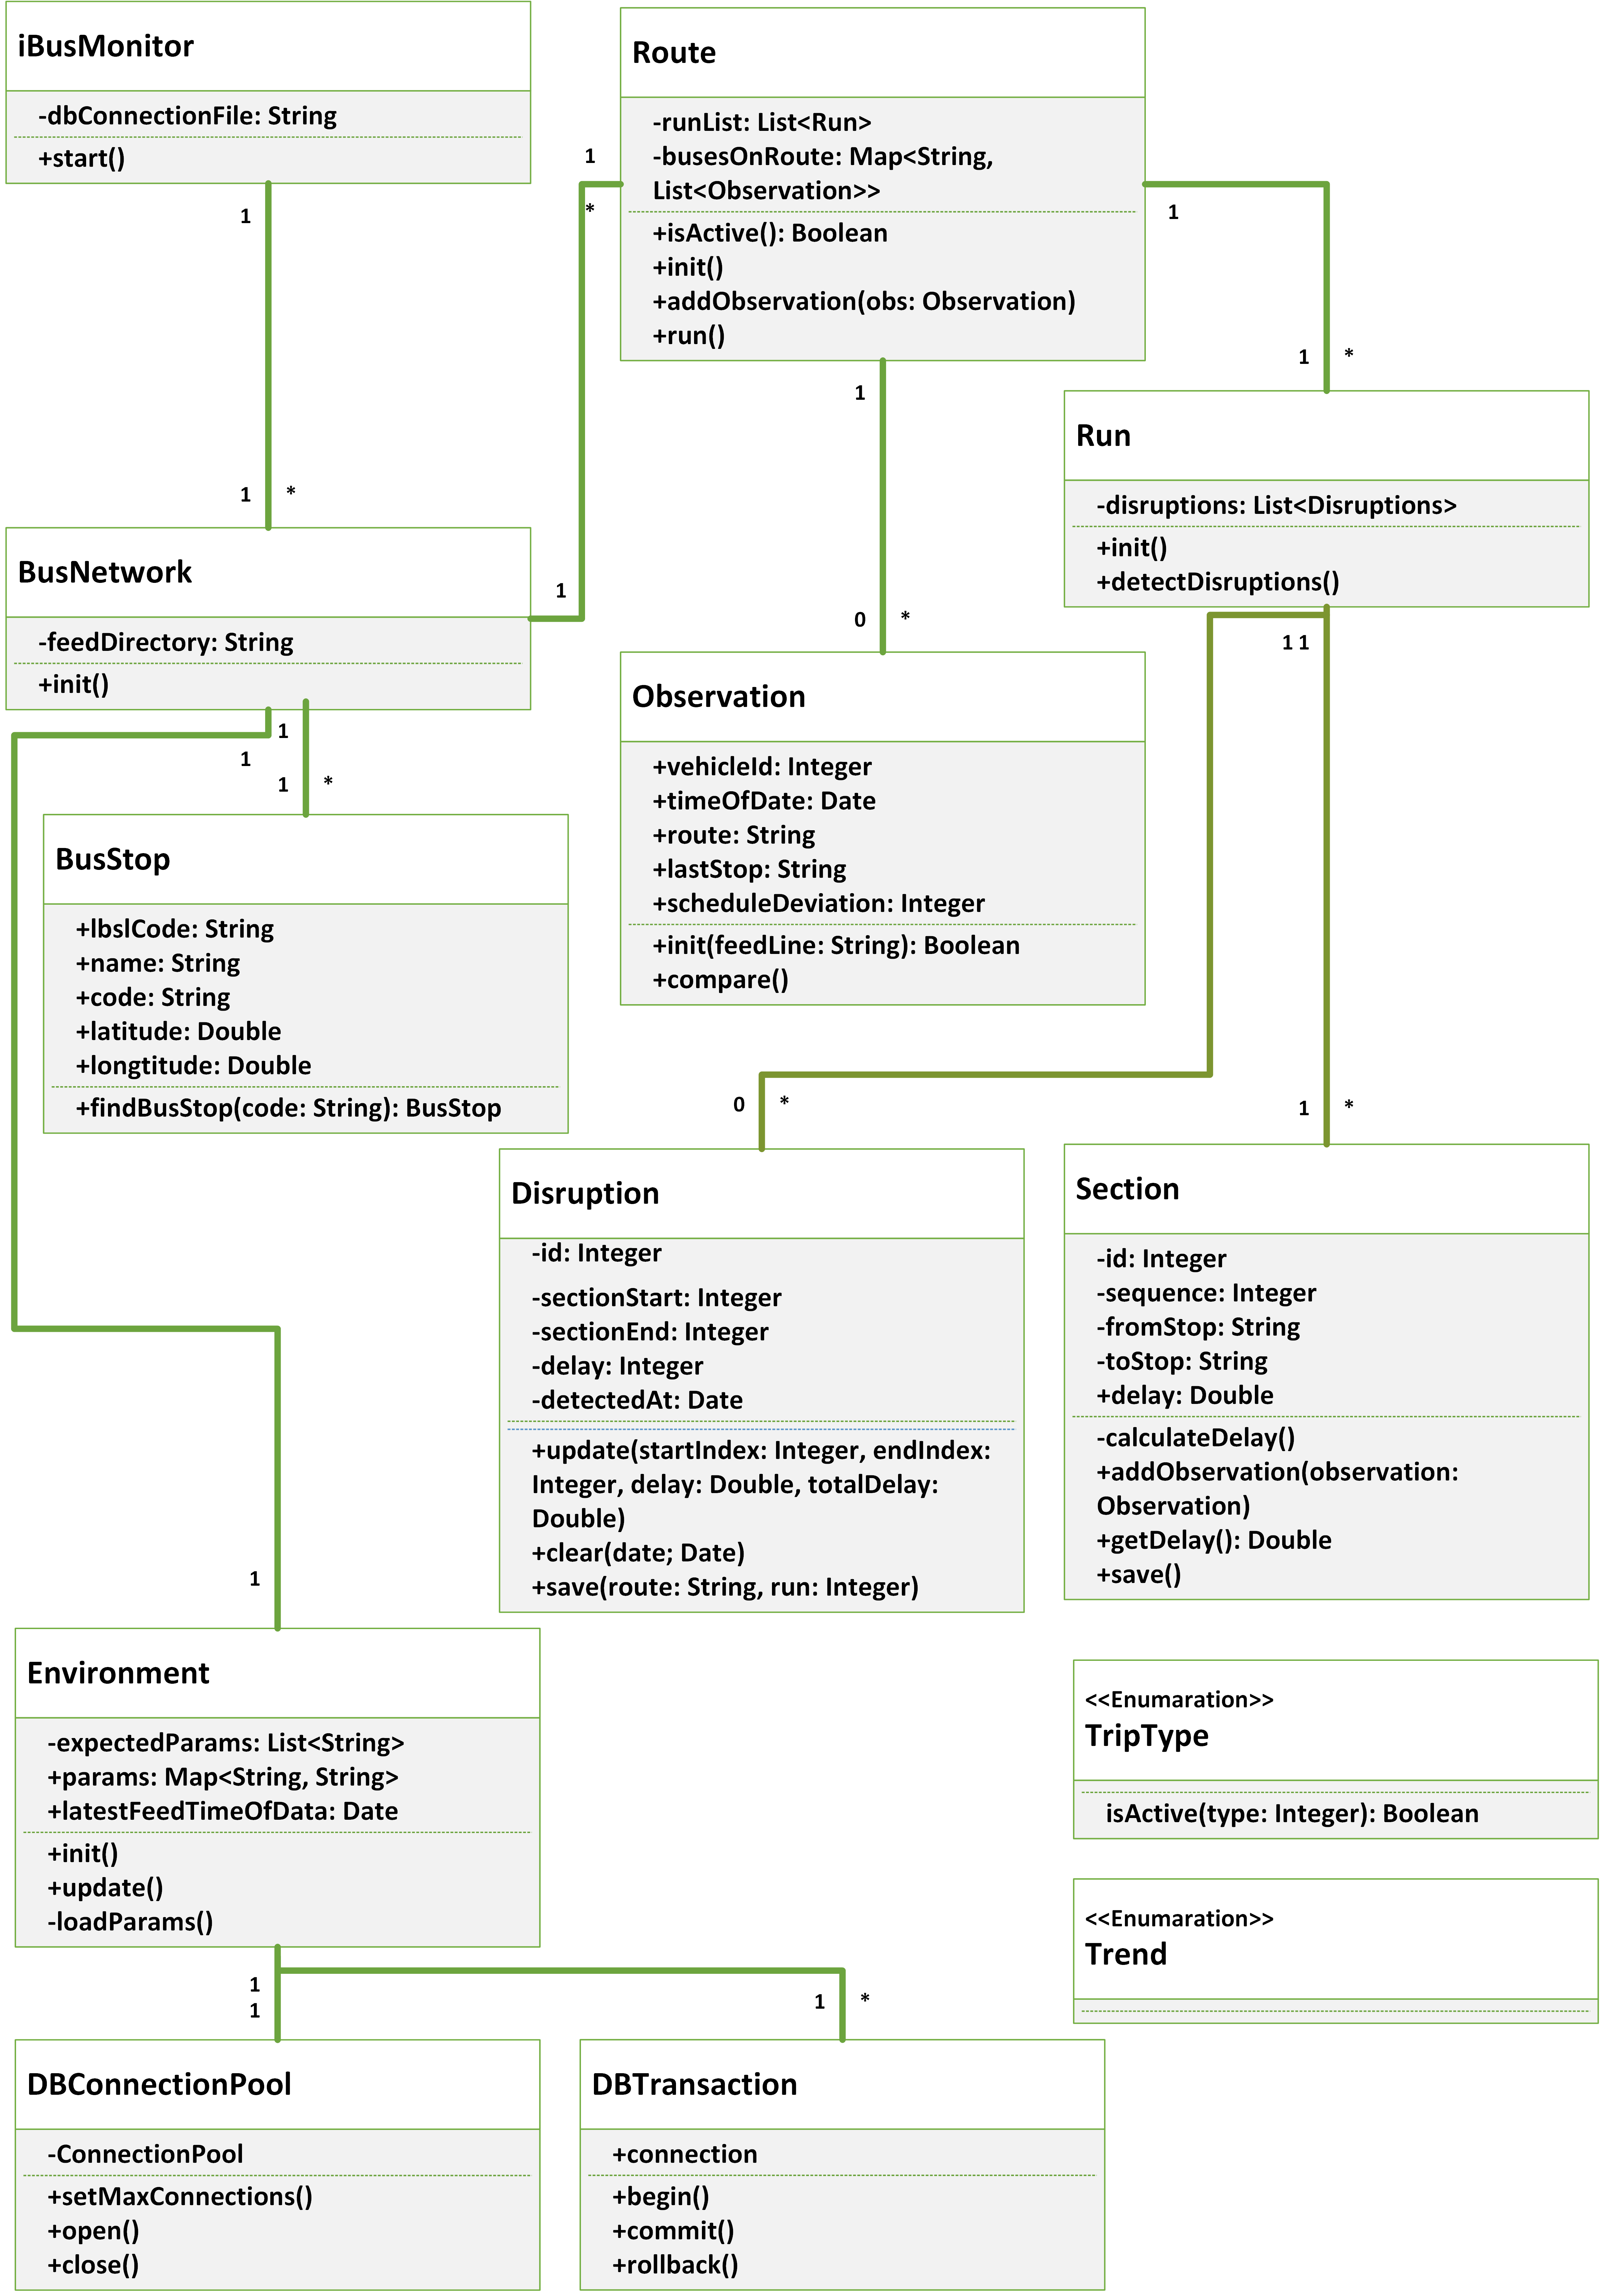
\includegraphics[width=1.2\textwidth]{Figures/Class.png}}
	\caption{Class Diagram}
\label{fig:class}
\end{figure}

\FloatBarrier
\section{User Interface}
The user interface of our system is addressing the second main aim of this project the one of visualising the calculated list of delays. The design and rational behind the user interface has been developed throughout discussions and meetings with CentreComm staff. The main requirement for the design is to be easy to identify the most important issues in the network. One of the uses of the user interface would be on a large monitoring multi-screen video walls which to be used not only by CentreComm, but by Traffic Management and even the Metropolitan Police. Another usage would be by the individual operators to access it through their personal computers. 

The above use cases and requirements have led to the decision of using a web-based application for the purpose of satisfying them fully. Using web rather than a standalone application, we allow for our system to be accessible from any device capable of running a browser (e.g. computer, laptop, smart TV, smart-phone, tablet etc.). Another advantage is that we only need to deploy the web application once and it can be universally accessed through the local network or even through the internet.

In order to improve separations of concerns we have also decided to have separate application for the disruption engine and the user interface. This means that we can change each one without affecting the other (considering we maintain the correct interfaces). This also allows us to implement and add more user interfaces apart from the web application if needed. For example we may even later want to create a dedicated mobile (tablet or smart-phone) application using the output from the disruption engine. This separation also allows to have different dedicated specialised people for maintaining each of the applications.

We have decided to use tabular approach for visualising the prioritised list of disruption. Each entry in the list would give detail of the route and section which are delayed. It also provides the time when the disruption was first detected. Any additional information is only provided on request from the user.

The overall architecture of the structure of the user interface can be seen in the architecture diagram in figure~\ref{fig:systemArchitecture}. An early mock-up of the graphic user interface can be seen in figure~\ref{fig:guiProposal}. This has however evolved a lot throughout the project. In Chapter 5 below we will give detailed description of the implemented visualisation and show the end user interface.


\begin{figure}[ht]
	\makebox[\textwidth][c]{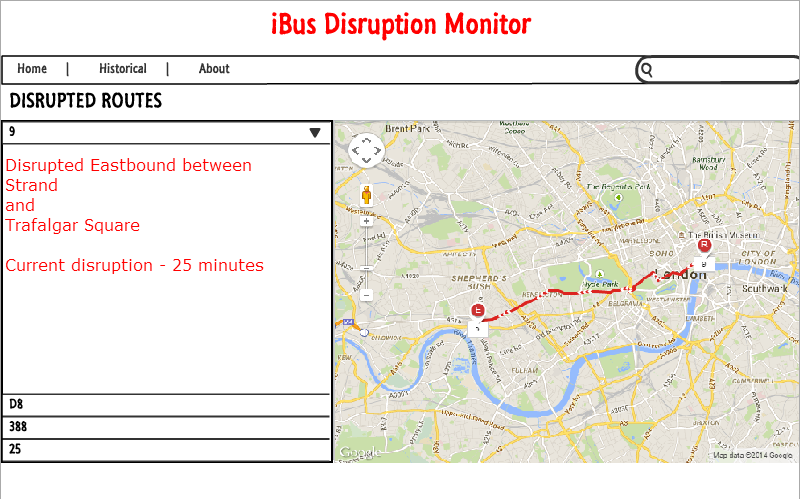
\includegraphics[width=1\textwidth]{Figures/guiProposal.png}}
	\caption{Initial GUI mock-up}
	\label{fig:guiProposal}
\end{figure}
\chapter{Implementation}
This chapter aims to present the reader with explanation of the key implementation aspects. These include major challenges, problems that have been encountered and decisions that have been taken during the course of this project. I have tried to avoid going into too much technical details except where this is essential and provides the reader with better insight and understanding of the material.

The system I have developed as a prototype which to satisfy our aims consists of two sub systems. These are the disruption engine which address the first aim of detecting disruptions in the bus network, and a web front end application which to visualise the calculated disruptions. Below I have presented the major implementation decisions and challenges that were faced during the development of this system. We begin with first describing the data that has been provided by TFL for this project. Afterwards we go into discussion of the implementation of the disruption engine which captures the core functionality and business logic of the system. Then implementation of the visualisation part is discussed which can be viewed as an extension of the disruption engine.

\section{iBus AVL Data}
%Include a sample of the data and explanation of all fields
%Explain what the schedule deviation value means
%Include discussion on how the network is represented and the source of the file - TFL open data
%iBus system generate very short telegram messages with the bus location \cite{Hounsell201276}. This information is then processed on a server and more information is calculated and derived.
%The data that has been provided by Technical Service Group (TSG) at TFL for this project consists of preprocessed iBus feeds. This feeds currently are being generated every 5 minutes. Each file consists of the following fields:
%The information we are interested is the deviation from the schedule. This is calculated by knowing the expected arrival time of the bus at a stop from the schedule and is compared to the observed time. This value is calculated the same way for both low and high frequency buses(Low frequency buses are supposed to run according to a fixed schedule (e.g. a bus should arrive at stop at predefined time) and usually routes which have less than 5 buses an hour. High frequency bus routes should maintain headways - this meaning a bus should be arriving at stop at predefined intervals (e.g. each 2 minutes)). More about the supplied data for this project would be covered in the requirements section.
%Key property of time series data is stationarity. This means that the behaviour of the time series data does not change over time. In our case the data generally speaking the time series data is not stationary. However if we consider short window size it might be possible to treat the data as close to stationary.
The data that is used for this project is provided by the Technical Service Group (TSG) at TFL. This data consists of comma separated value (CSV) files. There is an individual file for every different bus operator which contains the data for all buses currently operated by this company. Initially every bus in the network would transmit its unique identification number and GPS coordinates approximately every 30 seconds \cite{Hounsell201276}. This information is then preprocessed by a central server. This results in more information being derived, as the central server has knowledge of the whole network, the bus schedules and headways. This results in the CSV feed files that have been provided to us for this project. An example of the content of the raw feed file and a formatted version is presented in figure~\ref{fig:rawDataSample} and ~\ref{fig:formattedDataSample} respectively . Below I have provided a detailed explanation of each field in these files \cite{infoBusesInservice}.
\begin{itemize}
	\item \textbf{Vehicle Id} - this is a unique id of the vehicle.
	\item \textbf{Bonnet Code} - this is the bonnet code of the bus.
	\item \textbf{Registration Number} - this is the number of the registration plate of the bus. 
	\item \textbf{Time of Data} -  this refers to the date and time of when this data is received from the respective vehicle.
	\item \textbf{Base Version} - this the version of the system that is run by the respective bus.
	%\item \textbf{Block Number} - this is the block number on which the vehicle is running.
	\item \textbf{Trip Id} - stores the internal trips id
	\footnote{\label{loggedProperly}This is only valid when bus is properly logged.}$^{,}$\footnote{\label{routeVariant}Not available in route variant.}. This would increment every time a bus starts new run either at the end of its current run or somewhere along the run if it is curtailed.
	\item \textbf{LBSL\footnote{London bus services limited \cite{lbsl}} Trip Number} - this is LBSL trip number\footnotemark[\ref{loggedProperly}]. This is similar to the Trip Id however this is a global trip id thus it is incremented whenever a bus in the network start a new trip.
	\item \textbf{Trip Type} - the type of the trip as follows:
\begin{enumerate}
\item - From depot to start stop of the block.
\item - To new starting point.
\item - Normal trip with passengers.
\item - From the last stop of the block to the depot.
\item - Without passengers.
\item - Route variant.
\item - Vehicle not logged in either block or route.
\end{enumerate}
	\item \textbf{Contract Route} - the route name\footnotemark[\ref{loggedProperly}]$^{,}$\footnotemark[\ref{routeVariant}].
	\item \textbf{Last Stop ShortDesc} - this is the LBSL code of the last stop visited by the respective bus\footnotemark[\ref{loggedProperly}]$^{,}$\footnotemark[\ref{routeVariant}].
	\item \textbf{Schedule Deviation} - this is the standard deviation from the schedule, calculated using the bus position telegram, for the respective bus\footnotemark[\ref{loggedProperly}]$^{,}$\footnotemark[\ref{routeVariant}].
	\item \textbf{Longitude} - this is longitude of the place from where the vehicle is sending the telegram\footnote{\label{gps}GPS raw data divided by 3,600,000.}.
	\item \textbf{Latitude} - this is latitude of the place from where the vehicle is sending the telegram\footnotemark[\ref{gps}].
	\item \textbf{Event Id} - the last event Id.
	\item \textbf{Duration} - currently not being populated.
\end{itemize}

The information we are interested is the deviation from the schedule. This value is calculated the same way for both low\footnote{Less than 5 buses per hour.} and high\footnote{5 or more buses per hour.} frequency buses by knowing the bus schedule. It must be noted that it is possible for vehicles to have started the route run with some deviation from the schedule already.
%would start the route run already with some deviation from the schedule.

\begin{figure}[ht!]
	\makebox[\textwidth][c]{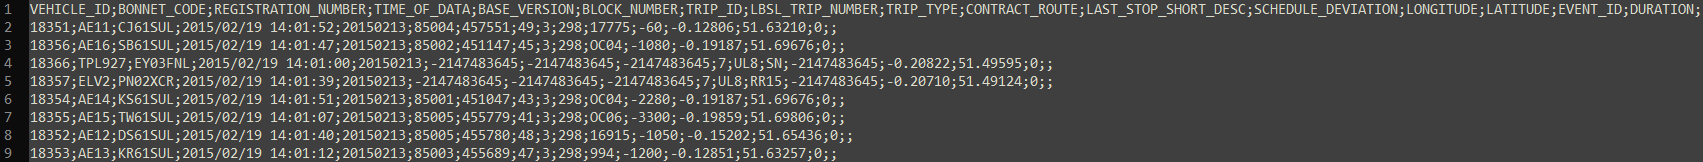
\includegraphics[width=1.7\textwidth]{Figures/ibusSampleRaw.png}}
	\caption{Sample Raw iBus Data}
\label{fig:rawDataSample}
\end{figure}

\begin{figure}[ht!]
	\makebox[\textwidth][c]{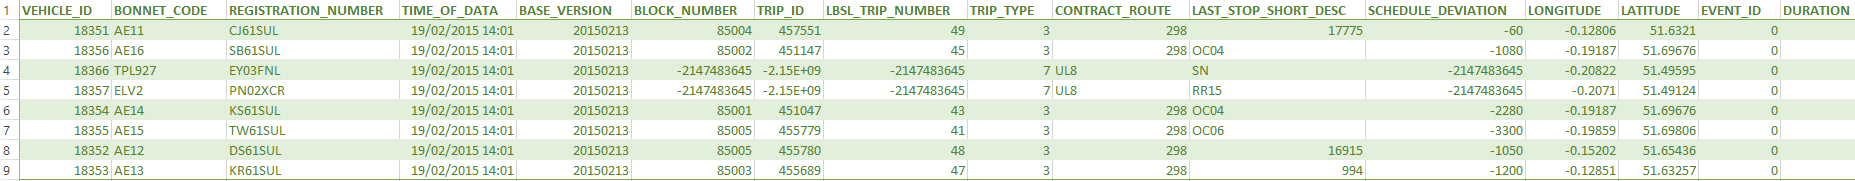
\includegraphics[width=1.7\textwidth]{Figures/ibusSampleFormatted.png}}
	\caption{Formatted Sample iBus Data}
\label{fig:formattedDataSample}
\end{figure}

\FloatBarrier
\section{Disruption Engine}
The disruption engine is implemented based on the design given in the previous chapter. The main implementation language used for the implementation is Scala. Scala is both functional and object oriented language \cite{odersky2008programming}. It is a type-safe Java Virtual Machine (JVM) language \cite{odersky2008programming}. This means that it is compatible with existing Java\footnote{\url{https://www.java.com/en/download/faq/whatis_java.xml}} code which allows for reuse of existing Java libraries. Scala was first introduced back in 2003, however, it has been only in the past few years that it had gained more popularity. In addition Scala enables the programmer to write more concise and clear code than one can achieve in Java. The decision of using Scala has also been influenced by the fact that I have good knowledge of the object oriented programming paradigm as well as experience in Java. This allowed me to quickly pick up and learn Scala and put it into use.

The disruption engine needs to have an accurate internal representation of the bus network. TFL's bus network and any other bus network usually consists of bus routes. Each bus route often has multiple runs (directions - e.g. inbound and outbound). In turn, each run consists of a sequence of bus stops that the bus passes through. In addition to these typical bus network components, for our implementation we also have the notion of a section. By this we mean a pair of consecutive bus stops along a given run of a given route. In figure 5.1 below we can see an example for route 15 outbound where we have depicted two section X (between Leman Street and Tower Of London Stops) and Y (from Tower Of London to Great Tower Street). This means that if we have $n$ stops on a given run then we have $n-1$ sections on the same run.

\begin{figure}[ht]
	\makebox[\textwidth][c]{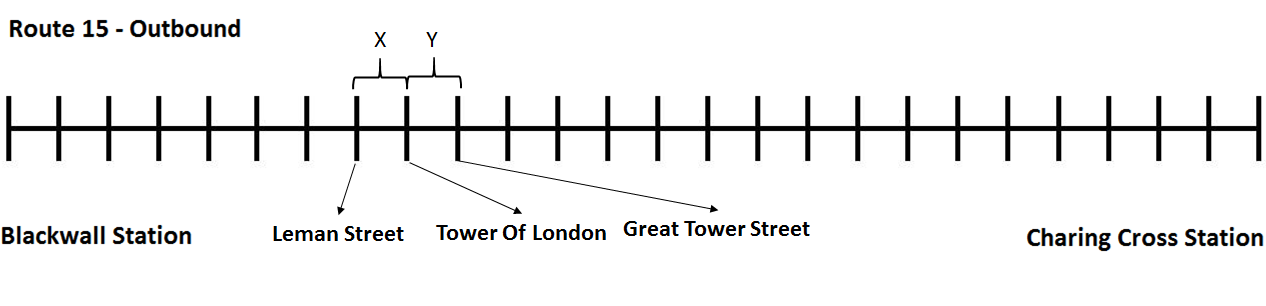
\includegraphics[width=1\textwidth]{Figures/sectionExample.png}}
	\caption{Example of a section}
	\label{fig:sectionExample}
\end{figure}

Our tool makes use of a PostgreSQL\footnote{\url{http://www.postgresql.org/about/}} database for storing all configuration parameters and also for storing the required information for the bus network representation. In figure~\ref{fig:dbModel} below, I have presented the relational model on which the database is based. The initial versions of the prototype used a CSV files as a means for storing the output. The decision to switch the flat file storage for a database is based on a number of things. The most important being is that using a database rather than CSV files we could keep historical data of the detected disruption for future analysis which is accomplished much easier using a proper database. Another advantage for the database approach is that it offers better concurrency support out of the box. Unlike the flat files which if manipulated concurrently could result in inconsistent state. Also having a database means that our disruption engine would require only details for establishing a connection to the respective database where it can read all other information that it requires. Otherwise it would require a number of other files and parameters to be defined which is not as easy to maintain as having one single database containing all of the configuration parameters, as well as data for the bus network representation. For the above reasons I have decided to use PostgreSQL as it is advanced open source relation database management system. PostgreSQL has very good document and community support which is a big advantage of any technology. Another advantage of using PostgreSQL for our implementation is that it ensures reliability and data integrity \cite{lerner2007open}. Also it supports Listen\footnote{\url{http://www.postgresql.org/docs/9.1/static/sql-listen.html}} and Notify\footnote{\url{http://www.postgresql.org/docs/9.1/static/sql-notify.html}} functionality which could be used for real-time updating of the web application along with Server Sent Events (SSE) \cite{serverSentEvents}.

%However as other research has pointed out \cite{1251929} calculating travel time as measure for congestion is difficult task and it is very dependable on the environment and its conditions (e.g. weather, time of day, public demand etc.). For this reason and because of the data available this project would not try to measure disruptions by calculating travel time or bus speeds.TFL has provided us with example of the AVL data which among other things contains a the GPS coordinates of the bus at a given point in time and preprocessed deviation from the schedule value. For the rest of this chapter we assume this value is accurately calculated and that we would receive this value for each bus in the network at some regular interval. The provided data is discussed in further details in Chapter 5.
%For this project we monitor and measure the schedule deviation value as calculating the congestion is very challenging and still not very well understood in the case of arterial urban traffic.
%However from the literature \cite{1251929} we can see that it could be difficult to precisely define what we mean by congestion in a transport network. It seems that congestion could mean various things to different studies and people.
%What is the general approach I have taken
%WHAT ARE THE CHALLENGES AND HOW WERE THEY OVERCOMED
\begin{figure}
	\makebox[\textwidth][c]{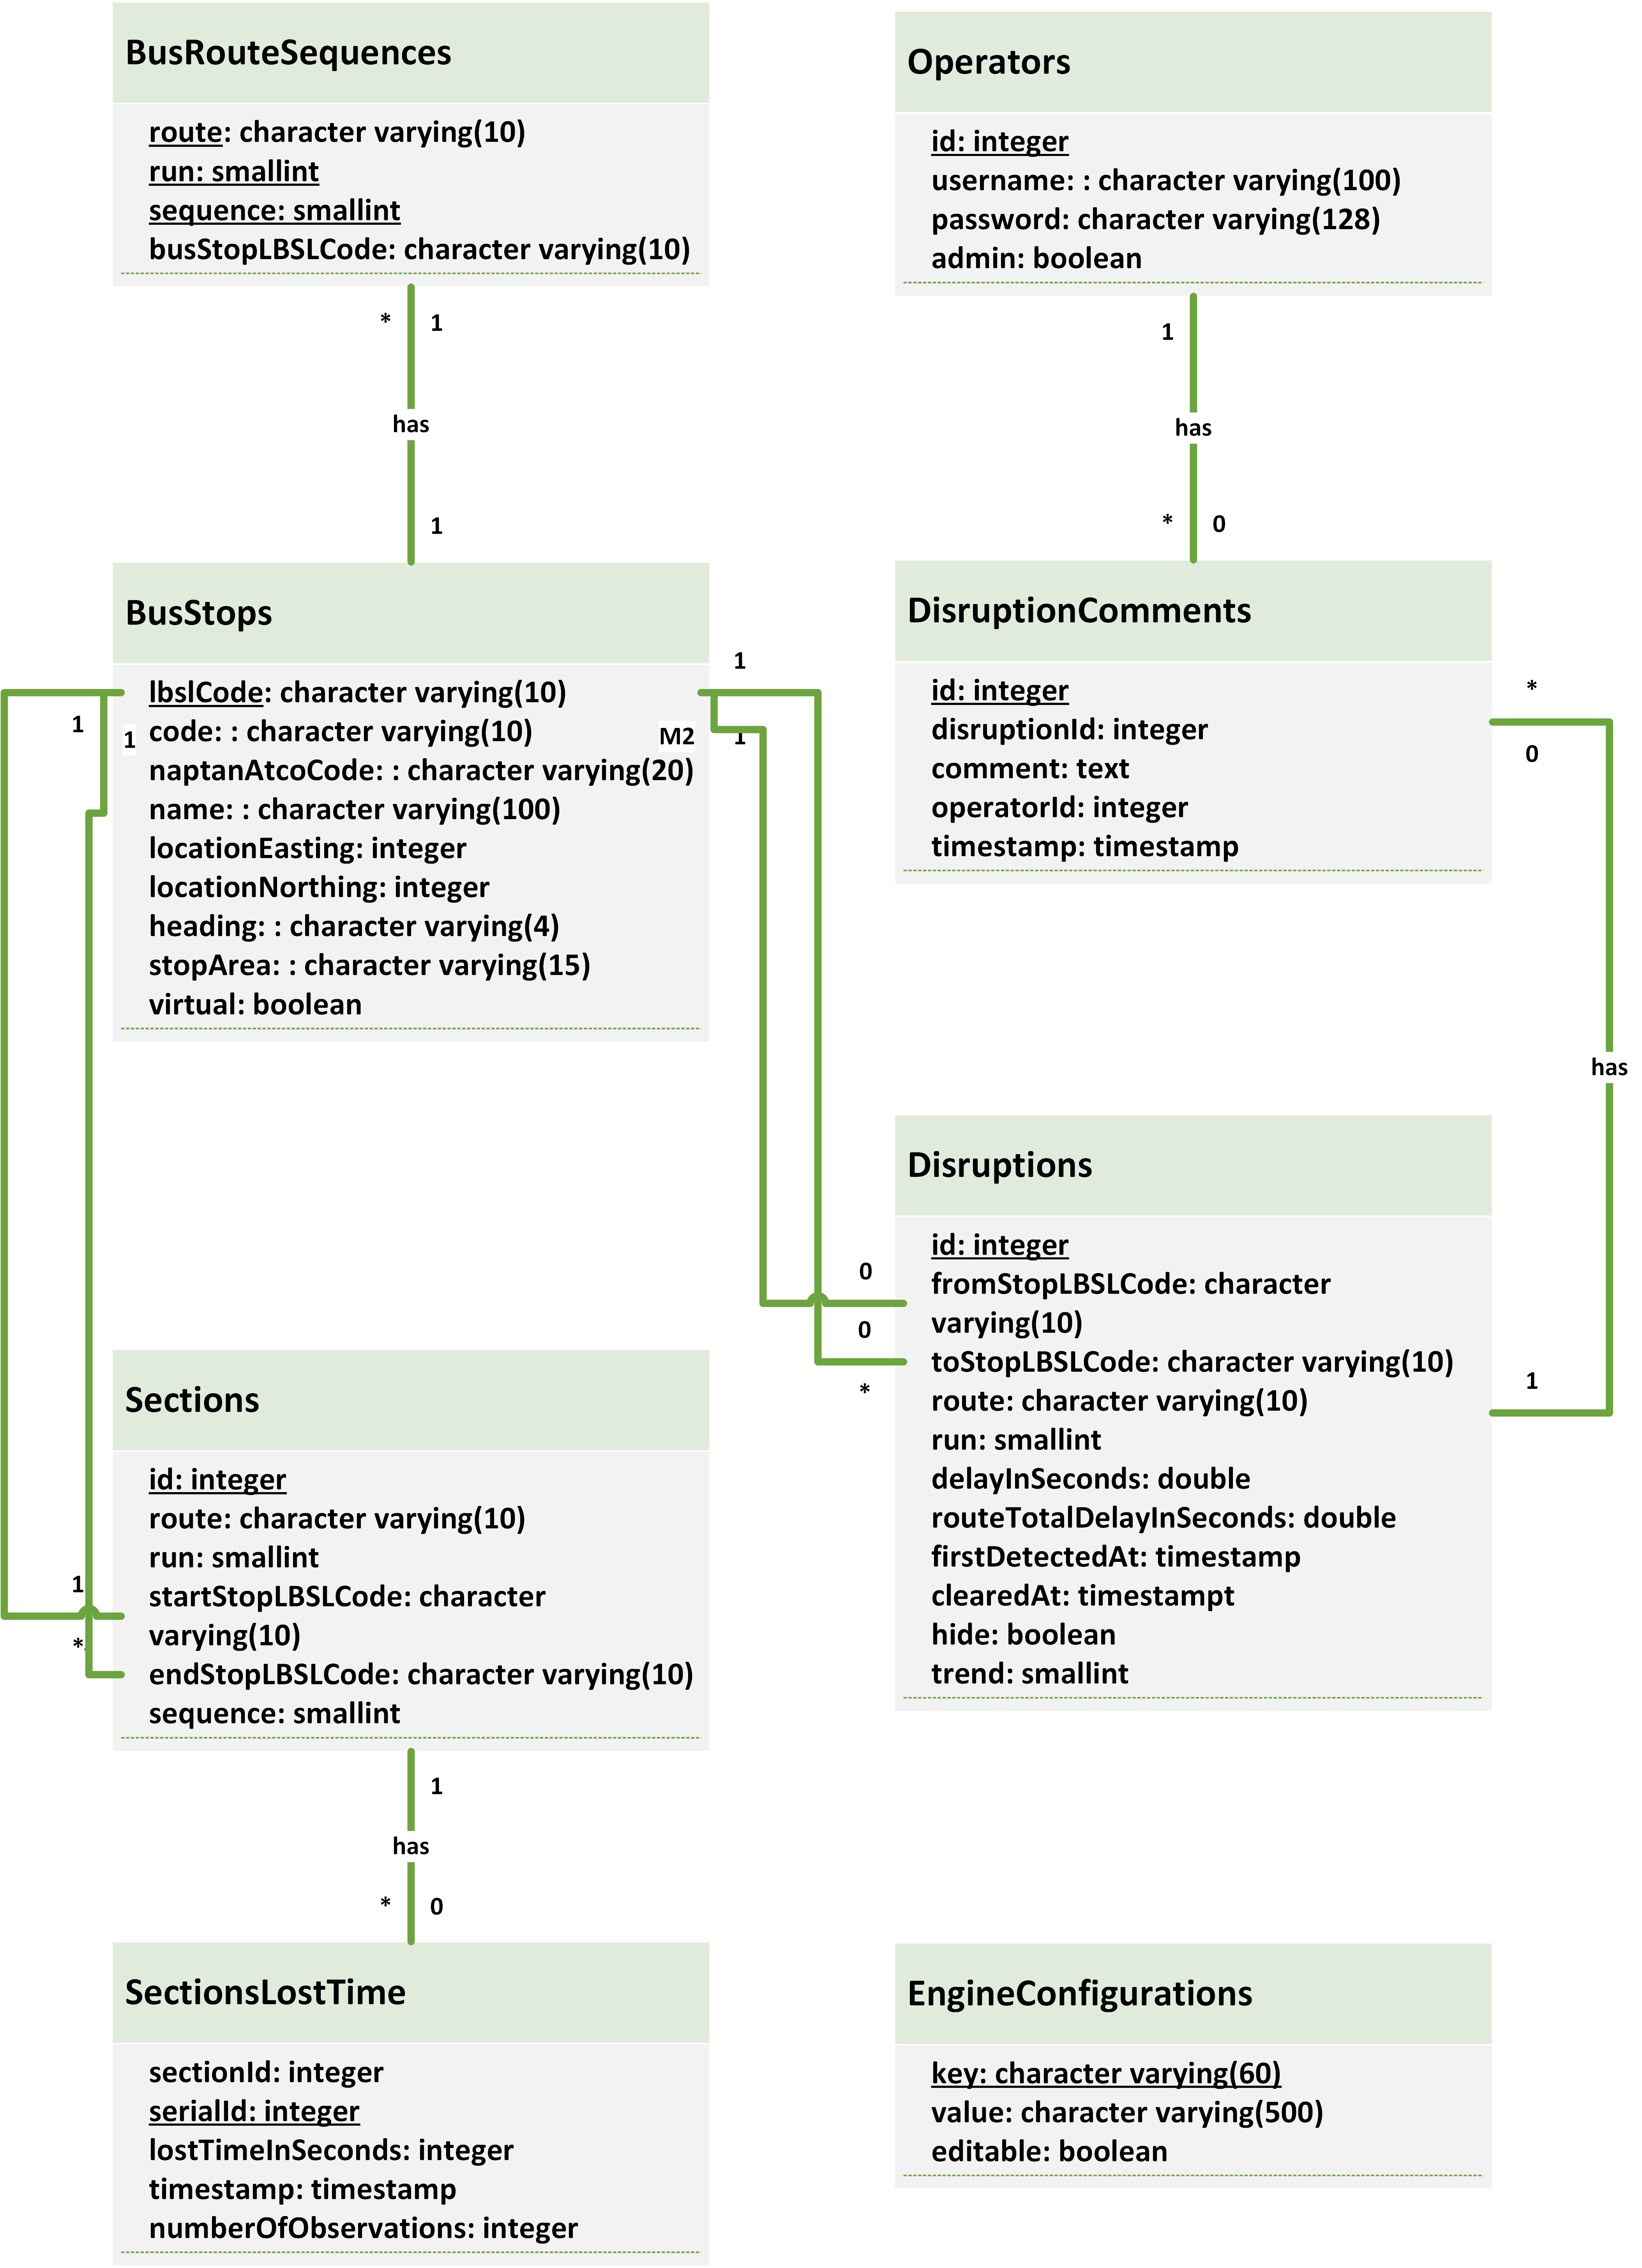
\includegraphics[width=1.2\textwidth]{Figures/DBModel.png}}
	\caption{Database Model Diagram}
\label{fig:dbModel}
\end{figure}

\FloatBarrier
\subsection{Bus Network representation}
In order for the engine to have full bus network representation, it requires information of the bus routes and the bus stops in the network. This information is freely available to anyone on TFL website \footnote{\url{http://www.tfl.gov.uk/info-for/open-data-users/our-feeds}}. It consists of two CSV files, one containing information on all bus routes and one for all bus stops in the network. The bus file contains a list of bus routes respectively has one or more runs which consists of sequence of bus stops. In our implementation we assume that this information is preloaded into the database. This preload consists of simply extracting the information from the CSV files obtained from TFL website into the respective tables (BusStops and BusRouteSequences). In addition to this we need to preload also the sections which will allows us to store individual section information. Currently sections are being generated manually however, this could be easily automated, but this is not in the scope of this project as it is most likely that TFL already have an internal database with this information in which case our tool will only require pointers to the respective tables. Then once the engine is started, it would read and load from the database all bus routes and respective sections. This results in the BusNetwork class storing a HashMap which maps a bus route name to the corresponding Route object. In turn, the Route class maintains a list of all runs for the respective route. BusStop information (apart from the bus stop LBSL code which we use as an id) is only loaded from the database on request. This whole process is part of the initialisation of the monitoring tool along with pre loading some other environment configuration parameters from the database. It happens only once throughout the execution of the tool and takes place just after the engine is started.

\subsection{Monitoring and processing new feeds}
Once the system is initialised, the tool will continuously monitor a specified directory (configurable from the database) for new feeds being written (pushed). Once new feed files are detected, they are picked up and processed by the engine. The processing consists of extracting the data of interest and calculating the time lost by buses on average for each section. Extracting the data means reading the CSV feed file line by line. Each line would be a data (observation) for a given bus thus we associate each observation with the route that is currently logged on. Once the observations are extracted, they are sorted by the time of the data field and any data that is older than a given predefined threshold (e.g. 120 minutes - this is configurable) is discarded. Once a given feed file is processed, it is moved to a predefine processed feed directory. This completes the feed file processing step. Feed processing is performed on batches of feeds (see the state machine diagram on figure A.5 in Appendix A). This means that once the engine detects new feed(s) in the directory it is currently monitoring, it will process all new feed files. 

\subsection{Bus network state update}
Once feed processing has finished, the system needs to update the bus network state. This consists of a number of steps. First we need to calculate the lost time per section. This process is done iteratively for every route in the network that has active buses (readings have been transmitted in some predefined interval of time e.g. 90 minutes). Each bus observation is then taken on a given route (see Figure~\ref{fig:example1}). At least two or more observations are required in order to calculate the time loss for a section. In the example below (figure~\ref{fig:example1}) we can take the first reading $x_1$ and the second reading $x_2$.
\begin{figure}[ht]
	\makebox[\textwidth][c]{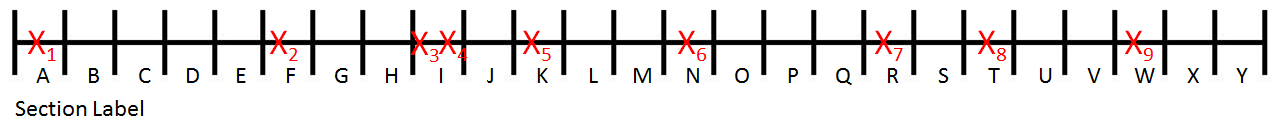
\includegraphics[width=1\textwidth]{Figures/implementationExample1.png}}
	\caption{Example of observations}
	\label{fig:example1}
\end{figure}
The difference in the schedule deviation between $x_2$ and $x_1$ is then calculated (see table figure~\ref{fig:example1Table}). 
\begin{figure}[ht]
	\makebox[\textwidth][c]{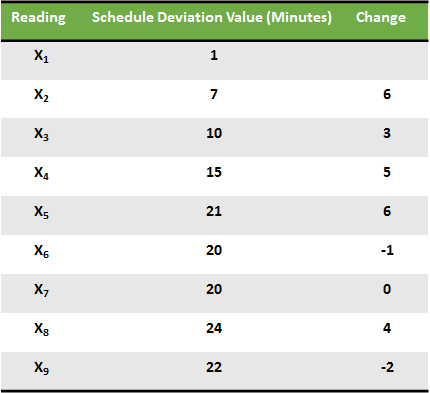
\includegraphics[width=0.8\textwidth]{Figures/implementationExample1Table.png}}
	\caption{Example schedule deviation calculations for the example in figure~\ref{fig:example1}}
	\label{fig:example1Table}
\end{figure}

Once we have calculated the schedule deviation change between two consecutive stops, we need to assign it to the respective sections. From our example we can see that reading $x_1$ has been sent somewhere from section $A$ and that $x_2$ from section $F$. This means that the bus have travelled through 6 sections ($A$ to $F$) and during that time it has lost $6$ minutes. The problem is that we do not know where exactly this delay has happened. It is possible that there was a delay just in one of the sections or it could have been distributed among all or few sections. For this reason what we do is to distribute this lost time evenly along all sections in-between the two readings. In our example this would mean that we would assign $1$ minute to each of sections $A$, $B$, $C$, $D$, $E$ and $F$. Then we take the next pair of observations, in this case $x_2$ and $x_3$ and do the same procedure. Every time we have new time loss value for a section, we add it to the existing lost time for the section and associate it with the newest observation time of the data. In this case that means section $F$ will have time loss value of $1+\frac{3}{4}$ and time-stamp equal to the time of data of observation $x_3$. If we however, take the case of reading $x_3$ and $x_4$ we know for sure that the delay has occurred in section $I$ thus we assign the $5$ minutes lost time only to section $I$. Repeating the above steps for each bus on a route will result in a list of values representing the delay (time lost) and the time (time of the data of the latter observation in the examples given above this means we take the time of the data of $x_2$ and $x_4$ respectively) when this has occurred.
 
Once we have a list of these values for each section of each bus route, we need to calculate the weighted moving average of this data. To do this we firstly need to sort this list of values for each section of a route run by the time of the observation in ascending order. Then we calculate the weighed moving average by assigning the oldest data weight of $1$ and the newest data weight of $n$ ($n$ is the number of data entries of a section). Calculating the weighted moving average instead of a simple average, we put more weight on the newer data and also help dampen the effect of a single irregularity (e.g. a bus has experienced a technical fault).

Doing the above steps, we obtain a value representing the WMA time loss (delay) for each section (see figure~\ref{fig:example3}). The next step then is to examine each route run and its sections in particular and check if any of them are disrupted. To accomplish this we firstly check if the total cumulative lost time of the sections of the respective run, is greater than or equal to some predefine minimal threshold (this is configurable). In case this does not hold (e.g it is below the minimal threshold) the algorithm will move onto the next run and will consider this one as clear (without any problematic sections). Any negative values (e.g where buses have gained time) are treated as $0$, as we are only interested if there are any problematic sections along the route run.

However if for example we assume that the minimal threshold is $20$ minutes and take the example from figure~\ref{fig:example3} we can clearly see that the cumulative lost time is greater than or equal $20$. In such cases we need to look more closely at this route run and try to identify the sections which are causing the most delay. We do this by searching for a number of consecutive sections which have their sum of the delay time greater or equal to some predefined threshold (e.g. 20 minutes). However, small delays (e.g of $1$-$2$ minutes) are treated as $0$ as there are always some slight variations and we are only interested in major disruptions which are beyond the control of individual bus operator companies. If we take the example presented in figure~\ref{fig:example3}, we can see that there seems to be some significant problem between sections $L$ and $O$. The sum of the delay is $7+14+12+5 = 36$ minutes which is greater than our example threshold of $20$ minutes. This results in the engine detecting and outputting a disruption between those sections.

\begin{figure}[ht]
	\makebox[\textwidth][c]{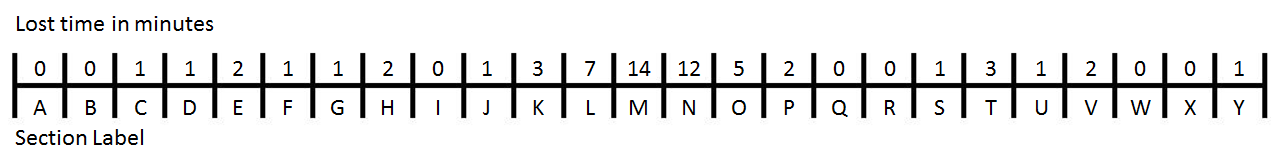
\includegraphics[width=1\textwidth]{Figures/implementationExample3.png}}
	\caption{Example of a disruption}
	\label{fig:example3}
\end{figure}

However, we have to limit the number of consecutive section we look at a single time as for example we consider the below case (see Figure~\ref{fig:example2}). We can have a long route run with very small loss of time per section (as in the example below, of the order of $1$ to $3$ minutes) but overall they might add up to $20$ or more minutes in particular if the route run is long (e.g has 30 or more stops). This however, does not represent a single problematic hotspot and is responsibility of the bus operators to manage such cases and not CentreComm. For this reason our algorithm would mark the start of a disruption as the first section it encounters with a greater WMA delay value and it would continue expanding this specific disruption until it finds/reaches a section with value less than the minimal threshold for section time loss value or the end of the run. Then it checks if the total delay for the detected sections is greater than or equal to the minimal disruption threshold. If true, it outputs it as a disruption affecting those sections. This is done for the rest of the route run even if some disruptions are already detected at the beginning of the run of a particular route.

\begin{figure}[ht]
	\makebox[\textwidth][c]{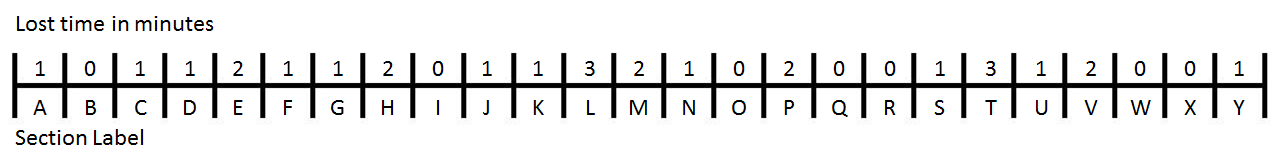
\includegraphics[width=1\textwidth]{Figures/implementationExample2.png}}
	\caption{Example of no disruption}
	\label{fig:example2}
\end{figure}

Every detected disruption or one such that it has changes in its state is updated and written to the database. This allows for the user interface to update itself with the latest information. The engine also writes a snapshot of the sections state of every route run in the network which has active disruptions. We only write data for the sections which belong to runs with disruption due to performance considerations. For example if we take the London bus network which has $680$ routes most of which have $2$ runs (outbound and inbound) and each run on average has $30$ stops, it means we have more than $40000$ sections. Updating them each time would take significant computational time (e.g. couple of seconds depending on the machine and the location of the database) and also would be waste of space. For this reason our implementation only updates sections which belong to disrupted runs as this information is utilised for displaying detailed graphs in the user interface.

%This is also the scenario where diversions become problematic.
%Once we have calculated the weight moving average time loss per section, we need to check if there are any sections that are of interested and need to be displayed (e.g. are there any disruptions).
%Here one problem arises as we need to take into account diversions. More details on this problem can be found in the section below. If we just ignore disruption we need to find if there is a number of consecutive sections which have their sum of the loss of time greater or equal to some predefined threshold (e.g. 20 minutes). For example in the example (see Figure 2) below we can see that section 5, 6 and 7 add up to 24 minutes of delay and thus we output that there is a disruption between stops E and H. 
%The next step is to calculate the weighted moving average of this data. We do this by taking the list for each section and sorting it by the time of the observation (e.g in the above example section 1, 2 and 3 would have time of the data equal to the x\textsubscript{2} observation).  
%Lets assume this difference is 3 and we can see that reading x\textsubscript{1} has been send from the first section of the route and reading x\textsubscript{2} from the the third section of the route. This means that the bus has lost 3 minutes between these two points on the route. However we cannot know for sure which section or sections have caused this loss and we can only distribute this loss equally between the three section. This means that each of section 1, 2 and 3 would be assigned 1 minute of loss. If we take however the case of reading x\textsubscript{3} and x\textsubscript{4} we can be very confident that the loss has occurred in section 5.

\FloatBarrier
\section{Graphical User Interface}
The engine implementation described above addresses only half of our requirements. In order to fully meet the project goals we need to be able to visualise the detected disruption in the network. For this reason we need to produce some kind of user interface which to be able to meet the requirements for visualisation of the detected bus delays. As described in section 4.5 of this report, we have decided to have individual application for the back-end disruption engine and the user interface. For the implementation of the user interface we have chosen to create a web application using Ruby\footnote{\url{https://www.ruby-lang.org/en/}} as the programming language running on Rails\footnote{\url{http://rubyonrails.org/}} framework.

The Rails framework is full stack open source web framework implemented in Ruby which allows for quick development and deployment \cite{guide2006agile}. It is relatively easy to use and maintain and it supports a wide range of software engineering paradigms and patterns. The main ones being Model View Controller (MVC), Don't Repeat Yourself (DRY), Convention Over Configuration (CoC) and the Active Record pattern \cite{fowler2003patterns}. Ruby is object-oriented scripting language which is famous for its conciseness. It enables the programmer to express his intentions quickly in very few lines code and it is also easy to read this code later (in future). Another advantage that Rails framework provide is the automatic code generators which provide code skeletons which save effort and time. Rails also allows for agile software development as this is in its roots \cite{guide2006agile}. It is also important to note that Rails has a strong support community and documentations as well as expansive list of add-ons and third-party libraries.

Other languages and framework have also been considered to be used instead of Ruby and Rails for this project. However, the chosen ones provide us with technologies which are to be used for quick prototyping and agile development which our project is following. In addition to the above this was also an opportunity for me to learn a new language and framework which I have not used before.

I have also made use of Foundation \footnote{\url{http://foundation.zurb.com/}} Cascading Style Sheets\footnote{\url{http://www.w3.org/Style/CSS/Overview.en.html}} (CSS) front-end framework. This framework has enabled quick prototyping as it has a rich library of predefined components. However, its main advantage over some other similar frameworks is its notion of grid which allows for quick and easy implementation of responsive websites. Making the web application with responsive design allows us to reach more platforms and client systems with a single application. This allows us with little additional implementation effort and time to achieve results which look good on both large screens (desktop computers, laptops etc.) as well as on small screen and mobile devices (e.g. smart phones, tablets etc.). This framework also has the advantages of good support in terms of documentation and add-ons and it is lightweight.

%Sample of what the system user interface looks like can be seen in appendix A [REFERENCE TO APPENDIX]. 
%For this reason I have decided to implement the visualisation part of the system as a separate web application. The advantages of this approach are that this provides universal access to the information. We only need to deploy this application once and it can be accessed from multiple clients running different operating systems and even devices. I have decided to use Ruby running on Rails framework. The reason for this is its recent popularity and wide support in terms of third party libraries and community information and guides.
%The Rails framework [REFERENCE] is full stack open source web framework implemented in Ruby.

The ruby on rails web application is implemented following the MVC pattern. MVC allows the programmer to structure their application code better with clear separation of concerns. In our case it consists of few simple models representing the corresponding database tables, controllers and a number of views. The models are implemented as Active Records\footnote{\url{http://guides.rubyonrails.org/active_record_basics.html}} which provide interfaces to the respective database tables. They provide create, read, update and delete (CRUD) functionalities. The controllers are responsible for processing the client request by parsing and checking for any parameters, credentials where necessary and responding with the requested information. The responses are, in most cases rendered views containing the requested information.

The user interface can be seen in figures~\ref{fig:ui1} to~\ref{fig:ui10}. It consists of three main views which are the disruption view (figure~\ref{fig:ui1}), the history view (figure~\ref{fig:ui3}) and the settings view (figure~\ref{fig:ui8}). The main view is the disruption one which is responsible for visualising the disruptions in the network at any point in time. The list is displayed in tabular form (figures~\ref{fig:ui1}). This provides instant awareness of what the network state is to the CentreComm operators. Disruptions are prioritised by their severity and are colour coded.

The application also has a basic authentication in place which enables to distinguish between the three type of users as described in section 4.1. Guest users do not have to authenticate, but they have limited access meaning they have read-only view of the system. The system also allows users to login in (figure~\ref{fig:ui4}) and depending on their status they could either be operators or administrator users. The administrator users have full access to the functionalities which includes view of the settings and the ability to change them, this is not possible if you are guest or operator user. Logged in users are allowed to hide/show (the result is that guest users would not see hidden disruptions) disruptions (figure~\ref{fig:ui7}) and also to add comments (figure~\ref{fig:ui10}). All users including guest are enabled to request further information for a given disruption which includes a graph of the lost time on the disrupted route see figure~\ref{fig:ui2}. This graph is a combo chart\footnote{\url{https://developers.google.com/chart/interactive/docs/gallery/combochart}} (combination of line and bar chart) and is created using Google Charts\footnote{\url{https://developers.google.com/chart/}}. The bars of the graph denote the WMA delay per section while the line depict the cumulative lost time along the route (this treats all negative values as $0$). The Google Charts API\footnote{API - Application Program Interface} allows us to make the graph interactive such that on hoover we can display more detailed information for the selected section which allows us to create a clear and organised layout with all the information available. This graph is very useful as it provides the CentreComm operator or other users with a detailed view of what is the state of the given route. The real-time disruption list and the history table are by default sorted by severity of the section delay and the total delay. However users are enable to sort by any other column. This is achieved using Ajax \footnote{Short for asynchronous JavaScript and XML} in order to minimise network load by only reloading the changed part of the web page (we do not need to reload the navigation menus, footers etc.). I have also added a data filter for the history view. The history view has not been part of the initial requirements or aims of the project, but it has been identified as great benefit tool like ours can offer. Because of this it has been added during the later stages of the project just as a proof of concept.

%The disruptions at any point in time are visualised in tabular form. Disruptions are prioritised by their severity and are color coded. Further details for disruption are displayed on request of the user. This includes a graph representation of the delay observed on each section along the disrupted route. On this graph the cumulative delay for this route is also visible. When hovered the graph displays details for this section including the start and end stop of it and the number of observations.

One important aspect of the user interface is how to update the disruption list in real time whenever there are changes. This is achieved by implementing Ajax short polling \cite{bozdag2007comparison}. This means that we use asynchronous JavaScript on the client side to make request to the server at predefined intervals. Alternative methods for implementing the updating of the list include WebSockets\footnote{\url{https://tools.ietf.org/html/rfc6455}}, Ajax Long Polling \cite{bozdag2007comparison}, Server Sent Events (SSE)\cite{serverSentEvents}. The main advantage of using Ajax short polling over WebSockets and SSE are that Ajax Short Polling is supported by all major web browsers natively unlike SSE which lacks Internet Explorer support. Also it does not require the set-up of any additional tools or infrastructure unlike WebSockets. The drawback of using Ajax polling is that in order to achieve near real time update, the clients will need to make frequent request to the server which wastes network bandwidth and server resources. SSE is the best approach in this scenario as it establishes a persistent long-term connection on which the server is able to push new data once it becomes available to all connected clients. However SSE is relatively new standard and it is has been standardized only as part of HTML5\footnote{\url{http://www.w3.org/TR/html5/}}. As mentioned above Internet Explorer does not support SSE and this is a major drawback in our scenario as this is one of the main web browsers CentreComm staff use. In addition to this, SSE require the use of a concurrency enabled server. WebSockets provide a persistent two-way connection between the client and the server however, in our case we are mainly interested in pushing new data from the server to the client. There is very little information the clients need to send to the server and thus we have excluded this approach as viable one.

\section{Problems}
During the implementation of the project a number of obstacles and problems have arisen. In this section we discuss the major ones. All that are not mentioned below are assumed to be solved by our implementation and not of enough significance for the reader.

The main challenge during the implementation has been how to assign the lost time between two consecutive observations to the respective sections that the bus has travelled through. This is because the data we work with is sparse (currently every 5 minutes) which means that during the time between those two observations the bus could have passed a number of sections and bus stops and we will only know the last bust stop it has attended. To solve this problem our the disruption engine keeps an ordered list of observations for each unique vehicle which is active on a given route. To assign the delays accordingly, the engine takes two observations at a time and does a number of steps. The first step is to check if the observations that have been made along the same run (e.g. both readings come from the bus when it was travelling outbound along the respective route). To do this we need check if the last stop from the earlier observation and the last stop from the latter reading are both from the same run and the earlier is preceding the latter last stop.

One problem that was encountered is that there is no explicit information in the data that has been provided if a bus is on diversion. Diversions vary greatly in terms of length (few or many stops) and duration (e.g. it can last half an hour or few weeks/months) of the implemented diversion. What happens in such cases is that the bus would still transmit its position, but the central iBus server would not be able to calculate the schedule deviation. This results in readings in the feed file which have abnormal values for the schedule deviation and other fields. These abnormal values however, are always the same and are equal to the negative integer $-2147483645$. However, this does not happen only when the bus is on diversion, it can also happen if there is problem with the GPS (e.g. weak signal due to high buildings) of the respective bus or if the bus is not logged on properly in the iBus AVL system. This means that we are unable to know for sure what such readings mean. For these reasons when such readings are observed by the engine they would simply be ignored. The implications of this are that our implementation loses some accuracy and it may produce delayed alerts. If we consider the example shown on figure~\ref{fig:diversion} where buses on this route are on diversion from section $F$ to section $P$, what will happen is that we will get correct data before and after the diversion which would be processed. However, during the diversion, the data we will get from the buses currently travelling on this diverted path will have meaningless values and thus the disruption engine will ignore it. This means that if buses experience delay during the diversion this would only be picked up by the system once they return on the normal route. However, the delay that the system will observe would be distributed along the whole diversion (as described above in section 5.1). This means that in case we have long diversion some significant delay might not be picked up by the system. This can also happen if there is problem during part of the diversion, but during the rest of the diverted route the buses actually manage to get back on schedule.

\begin{figure}[ht]
	\makebox[\textwidth][c]{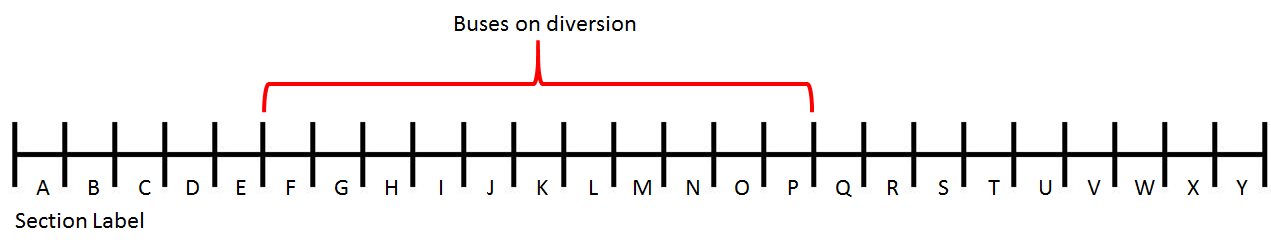
\includegraphics[width=1\textwidth]{Figures/diversion.png}}
	\caption{Example of diversion}
	\label{fig:diversion}
\end{figure}

Another problem with the available data is that we do lose some accuracy (some readings are ignored) when the bus turns at the end of a run. We cannot simply assume that every bus would travel along a route from start to end and turn as there are occasions when buses are curtailed\footnote{To cut short.} along the route. This can happen for a number of reasons including service regulation, heavy congestion/disruption along some sections of a route, bus driver exceeding the allowed by law work hours and more.

Our system relies on monitoring for changes in the schedule deviation value as indicator for the delays in the network. However, there are some scenarios where the engine can detect delays where in fact there are no real-life disruptions taking place. To understand why this can happen, consider the case when a bus is initially ahead of schedule. This can result in the bus driver or operator company to deliberately force this service to lose time in order to be right on time. This is especially a problem for low frequency buses as they run according to fixed schedule and not based on headways. Thus we can claim that our implementation provides an upper bound of the disruption delays in the bus network.

Another problem of the approach taken is that because the system relies on monitoring the schedule deviation value and it does not treat differently calculations where during the first observation the bus is ahead or schedule and when it is already behind. This means that it is possible that the bus driver is losing time on purpose for service regulations. Thus we can assume that our tool provides an upper bound of the disruption.

Some other problems with the implementation include inconsistencies in the bus route sequence data. This however, is affecting small number of routes and does not prevent our system from delivering a proof of concept. This issues have been discussed with members of the TSG and have been considered irrelevant for the purpose of this project. However, it has been agreed that they would need to be addressed in case this is tool is put into production. 

%When such readings are observed by the engine they would simply be ignored. This is problematic and our system only ignores it in the current prototype as failure in computing the schedule deviation could also be caused by the bus not being properly logged into the iBus system (e.g. bus taking a break at end of route). This means that we lose some accuracy especially for longer diversions as any lost time would be distributed along the sections which have not been observed (where the bus has been on diversion). This however could also be the case if a bus skips or fails to send data. Again this could be because of number of reasons (e.g. weak signal due to high buildings etc.).

%The important factors to consider are the weights and the period/window size to use. We could also apply exponential smoothing on top of the WMA.
%Problems:
%The bus could have started the journey ahead of schedule and thus to intentionally be losing time.
%The buses could curtail anywhere on a route without notification
%The buses could be diverted (this could be short term or long term) it can also be for few stops or it could be a longer diversion.

%PROBLEM - some buses might skip transmitting data even if they are properly logged on
%Data available, data frequency, no knowledge when buses do curtail, not taking into account bus dwell time, bus drivers who are running ahead of schedule could be driving slower on purpose and thus. Tool gives an upper bound of the of the WMA lost time per section. 

\chapter{Testing}
Testing is important and integral part of any software development project. It is necessary to carry out testing throughout the implementation as well as once the system is completed in order to make sure it functions correctly according to the requirements and the design.
%The disruption engine consists of a number of individual components and algorithms.These are tested using a number of unit tests. Due to the nature of the engine, stress tests were carried out to test it for any memory leaks and performance issues. Evaluation of the output of the disruption engine will be performed by first carrying out further literature review to find some guidance on what window for the data to consider to use and what weights to use for optimal results. This will be followed by running the system on a given set of data (e.g. a week worth of AVL data) and comparing the output with the actual state of the network during this period.

%The user interface consists of a simple web application capable of displaying list of disruptions. Testing and evaluation of this web application will be performed as user testing. As I mentioned above, some feedback and problems were identified which will be addressed and fixed. Follow up user tests will be carried out by giving access to friends and family to the web site to use and give feedback on. This should give reasonable confidence in the correctness of the user interface as there is no complex logic incorporated in the web front end application.
\section{Unit Testing} 
As described in the previous chapters the system is composed of a number of classes each of them representing different part of the bus network with its own functionalities and responsibilities. Throughout the development of the product a number of unit test have been carried out in order to ensure that each of the classes function correctly as per requirements and carries out the required task. Each module was tested separately before being connected to the rest of the system.

\section{White Box Testing}
Apart from the unit testing through the development of the tool we have made use of the debugging tool provided by IntelliJ IDEA\footnote{https://www.jetbrains.com/idea/} integrated development environment (IDE). This was the main IDE used for the development of this project (both the disruption engine and the user interface web application) and has provided many useful tools and support. The built-in debugger allowed us to carry out inspection of the code during its execution while still developing the application in order to make sure that desired outcome is produced. The debugging tool allows us to halt the execution (in real-time) at specific point during the calculations and examine the state of the program (the values of all variables). This has proved very useful as it allowed us to quickly fix and rectify any issues early in the implementation which otherwise could have remained hidden.

\section{Functional Testing}
Functional testing is type of black box testing. This is because we test the software product by feeding it some input and examining the generated output. Functional testing does not mean we are carrying out test on individual methods/functions or classes/components. It means that we are testing parts of the functionalities stated in the requirements. As our system consists of two sub systems we are able to perform separate functional testing of each of the systems.

The disruption engine was tested by having an automated functional tests which feed the system with a feed file and then examine the produced results. Some of the example test cases include:
\begin{itemize}
	\item Correct, but empty feed file is pushed to the system.
	\item Single correct feed file is pushed, containing a single bus reading.
	\item Two correct feed files are pushed containing a single bus reading from the same bus each.
	\item A malformed feed file is pushed to the system.
	\item A batch of feed files is pushed to the system.
\end{itemize}

The web application part of the system does not contain much complex logic. The most complicated part is that of retrieving the right data. This required some more complex SQL queries which were tested manually using and SQL editor program. However the rest of the functionalities of the user interface have been tested by me throughout the implementation. As the user interface is basically visualising the generated output from the disruption engine a two main scenarios have been employed during its testing. The first is testing the functionalities while the disruption engine is either not running or it does not produce any output. The other is while new output is being generated by the back end and the user interface is continuously updating itself. In addition to these scenarios due to the fact the system distinguishes between three type of user roles I have assumed each of the roles and carried out manual tests to verify the correct behaviour from the system. 

Some feedback has been received regarding the user interface during demonstration and discussions with CentreComm and my supervisor. All remarks and suggestions from the received feedback has been addressed. In addition to that I have asked family and friends to spend time and test the functionality of the user interface for this I provided them with a list of use cases and the expected behaviour. This has proved useful in identifying some issues with the functionality and the compatibility of the product with different web browsers and systems. All of the identified problems have been addressed and rectified after that.

%USER INTERFACE - this consistes of testing the user interface in live state (while the engine was generating more input and updating the state) and also at paused state when the engine did not run or did not generate any input. I considered all three user roles and tested the system for the expected output.

%This was carried out by manually testing the functionality of the web application and verifying that it resulted in the correct output. The user interface has been tested by me throughout development, some feedback has been received on it during demonstration and discussions with CentreComm and my supervisor. In addition to that I have asked family and friends to spend time and test the functionality of the user interface for this I provided them with a list of use cases and the expected behaviour. This has proved useful in identifying some issues with the functionality and the compatibility of the product with different web browsers and systems. All of the identified problems have been addressed and rectified after that.

\section{Stress Testing}
On of the main requirements for detecting the disruptions in the bus network is for this to be calculated in real-time. Because of this we need to make sure that the implementation is able to cope with large amounts of data quickly. Each bus reading we receive in the AVL feed file is on average $100$ bytes. There are could roughly up to $7000$ buses active in the bus network at each point in time. This means that the system should be capable of processing $1$MB of data every $30$ seconds as close to real-time as possible. Also as the system will run continuously with more data being pushed to the system throughout its execution it need to be ensured that any memory that is occupied by data that is irrelevant (old) be discarded appropriately without causing any memory leaks. 

The approach that I have taken in order to test the system for such performance issues consisted of firstly creating an automated script for simulating the feed pushing to the tool. This program takes two main input parameters. One is the directory in which the feeds for the simulation are being stored and the second main input is the rate at which these files are copied to the directory which is used by the disruption engine for monitoring. Currently as discussed previously in this report the AVL data files which were provided for this project are generated every 5 minutes. However this could be changed in future if the tool goes into production. For this reason we need to make sure that the proposed prototype is capable of dealing with all of the data that is being pushed to the engine every 30 seconds (as this is the current rate iBus equipped buses transmit data). Apart from the rate at which new data is pushed to the tool the performance of our system depends mainly on how much data is pushed (e.g. during the night ours there are less active buses thus less data generated compared to daytime) and also on how many disruptions are detected in the system. The earlier is clearly obviously that if there is more data to be processed the system would naturally take longer. However the second statement is because we only update the database information for a route, run and section only if there is changes. This means that the update time could vary greatly depending on the number of changes at each network update. In order to minimise the impact of this the system is implemented in such a way that it makes all database updates after a network update in one transaction. This means that the main performance bottleneck of the system becomes the updating of the database. The initial versions of the prototype did not make use of a database, but rather wrote the output into flat CSV files. The reason for adding a database in place of the flat files is that the implementation change, so that it could keep historical state of the network which could later be used for further analysis and reports which are features that have received a lot of positive feedback from TFL.

Simulations have been run to make sure the system is capable of processing and updating itself in real-time. This tests have been carried out on a laptop running Intel Core i7-3610QM with 16GB DDR3 1600Mhz of ram and Windows 10 x64 bit operating system. The simulations consisted of feeding the tool with a week worth of data that was provided by TFL. The data was made of 21629 separate (each one for a single bus operator) AVL feeds which have been group into 2814 batches according to their timestamps. The total size of the sample is 1.07 Gigabyte (1076394754 bytes) and the average size of a single feed file is 49.77 Kilobytes (49766.27 bytes). We ran a number of simulations with this data keeping all parameters the same and re-initialising the system before each run. The only parameter we altered, to make sure the system is capable of handling data at higher rates, is the rate at which the feed simulation program pushed the AVL files. The results could be seen on figure~\ref{fig:stressTestResults} below in this chapter. From the results we can conclude that even on a normal computer in a development environment the system is capable of producing output in almost real-time. The memory usage also could be seen in the results shown on figure A.10 in Appendix A. The memory was measured through the execution of the tool and readings were taken every minute. The memory usage is highly dependent on the amount of the data being processed and also depends on when the Java Virtual Machine(JVM\footnote{http://www.oracle.com/webfolder/technetwork/tutorials/obe/java/gc01/index.html}) garbage collector executes. The latter is because the system might have already removed all references to some object, however this memory would not be unallocated until the JVM garbage collector is called.

The system current implementation is updating each route in the network consecutively. However the system has been implemented with concurrent execution of this calculation in mind. This means that it could easily be updated such that each route is concurrently processed. This is also the case for the parsing of the CSV feed files and observation extraction. As the aim of this project is to built a prototype I have decided not to spend the limited project time on such optimisations as it is more important to prove if this is viable solution. As it can be seen from the stress tests carried out even without such parallelism in place the system is capable of  generating output in less than a second. This means that the bottleneck for achieving real time updates to the users is the user interface implementation (e.g. how often the client web browser will poll the server for updates).

\begin{figure}[ht!]
	\makebox[\textwidth][c]{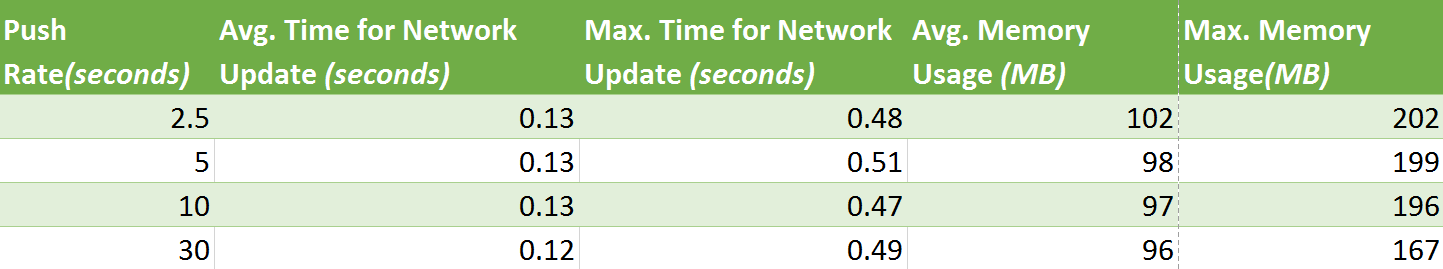
\includegraphics[width=1\textwidth]{Figures/StressTestResults.png}}
	\caption{Stress test results}
\label{fig:stressTestResults}
\end{figure}

%The results shows us that there are not problems with dealing with large amount of information in real time even on a normal mobile computer. It can also be seen that memory usage is within the capabilities of typical modern computer. We can see big variations in the memory usage, however this is normal as we do not explicitly allocate and deallocate memory. Scala runs on the Java Virtual Machine (JVM) which has garbage collector reponsible for freeing up unused memory. The only thing the programmer need to make sure for is that any objects that are unused should have no references pointing to them, then when JVM garbage collector executes it will return (free up) all unused memory. This means that our system memory usage depends on:
%\begin{itemize}
%	\item How fast new data is pushed.
%	\item How much data is being used (as discussed in the previous chapter).
%	\item How often the garbage collector executes.
%\end{itemize}
%Evaluates the artefact, comparing results expected from theory (including those for alternative designs) with those obtained in practice.
\chapter{Results \& Evaluation}
Evaluation is important step of every software project yet it is sometimes neglected. This chapter aims to discuss how and what evaluation has been done of the prototypical tool we have proposed and implemented. This is followed by discussing the results that were obtained during the evaluation.

%For our project we are only ably to objectively evaluate the performance of the disruption detection engine. Evaluation of the visualisation is very subjective and it will vary greatly between one user and another. For this reason we only rely on feedback from users especially CentreComm operator which we can use as a measure for the success of the particular visualisation we have implemented to complete this project. The disruption engine however needs to be properly evaluated. In order to evaluate it we need to answer three questions:
%What is being evaluated?
%How is it evaluated?
%What are the results have been obtained?
\section{Evaluation}

\subsection{Disruption Engine}
In order to evaluate and verify that our tool is able to detect disruptions we need to run the system with some data for which we know what the output should be. This means that we can analyse the output once the system has processed the sample input data. Analysing the data need to focus on whether the system is able to:
\begin{itemize}
	\item Detect all disruptions present in the data it is fed with.
	\item Detect and alert of those disruptions in real time (there is no or very little lag).
	\item Calculating accurate and reliable estimates of what is the actual (real life) state of the bus network.
\end{itemize}

However achieving this is problematic in our case as the data provided by TFL is only the real AVL feed files.
There is no formal information or list of all delays, their severity and duration for a given period of time. We have been provided with some links to web blogs which contain some of the diversions that are being implemented on daily basis in response to disruptions in the network. However, we cannot formally use this data to evaluate our product as this is neither an exhaustive list nor precise and accurate source of information (the delays stated there vary greatly and are somewhat subjective). We can analyse the provided bus feeds manually for a given period to extract what the actual state of the network was during that time. However, if we want to cover a number of scenarios this approach becomes infeasible as it will require great effort and time which are limited. And if we want more cases for evaluation it will require us to go over and repeat the same process again and again.

In order to overcome this problem we have decided to generate some test data on our own. We have achieved this by implementing a simple program for generating iBus AVL-like feed files. This allows us to compile test data with different scenarios and test if our system achieves the expected results. We have limited our test data to four scenarios as follows:
\begin{enumerate}
	\item The schedule deviation value remain fairly constant with very minor changes across the route for every bus on that route. This scenarios should yield no disruption detections.
	\item Single bus incident (e.g. bus breakdown, customer incident, error reading etc.). This again should not be picked up by the system.
	\item General traffic scenario. This means that there is gradual schedule deviation increase at some point of the route run. This is the most typical real life scenario (e.g. rush hour traffic build up) and it should be detected by the system.
	\item Incident (e.g. traffic collision) along a route. The data for this would represent a sudden increase in the schedule deviation. This needs to be detected by the tool.
\end{enumerate}

Once we have generated the data for the above scenarios, we need to run the system and feed it with the artificially generated input. We run each of the above scenarios separately and the system is re-initialised before each run. This allows us to have the system in the exactly same state for each test.

These tests allowed us to run multiple simulation in order to adjust the weighted moving average parameters. These are the weights and the moving average window. This parameter values are critical for the accuracy of our tool. They have direct impact on what is being detected by the tool and with what lag. We also altered the data validity parameter which represents when we discard any observations.

In order to calibrate our prototype and its output we ran a numerous simulations with the describer scenarios and different values for our parameters. Using our test-generated data we have obtained best results with having the data validity set to 90 minutes and the moving average window size equal to 5. This means that we only consider the last 5 observations for a given section which have occurred in the last hour and a half. We also use weight of 1 to 5 (1 for the oldest and 5 for the most recent). This allowed for a balance output, as the system tended to overreact if we used an exponentially growing weights or it lagged behind if we used a greater moving average window. Also keeping data for the last 90 minutes in memory should work well for both low- and high-frequency buses, as from the data provided we do not have any indication of the type of the service. This however, needs to be further tested and evaluated by either generating further test data or using real AVL data for which the bus network state at that point is know.

%In order to check if the system we have proposed can satisfy those requirements we need to run simulations and check if they result generated by the prototype match our expectations. One option to accomplish this is to use real data that was provided by TSG of TFL. However the problem with this approach is that we do not have a complete list of what was the actual state of the network at that time (the period of the sample data provided). It would be infeasible for us to manually analyse it in order to calculate what, when and for how long it should be picked up. This leads us to the seconds option which is to manually generate some test data which conforms to the iBus AVL data.

\subsection{Visualisation}
The web application part of our system was evaluated by simply using the list of requirements. Using the defined requirements from Chapter 3 of this report we were able to verify that all expected functionality is in place and produces the correct results. This also included testing that the application is behaving and displaying the same way on the most widely used browsers (Internet Explorer, Firefox and Chrome) as well one some mobile devices (Android tablet, Ipad and Iphone). All of the test verified that the system is consistent across the various devices and no functional issues have been identified.

\section{Results}
During the testing and evaluation of the proposed prototype we have ensured that all user and functional requirements have been met. Our simulations using artificially generated data proved that the proposed system is capable of effectively monitor changes in the schedule deviation value. However, further evaluations and analysis is required into whether using this values provide us with an accurate and reliable measure of the actual delays in the bus network. As it has been discussed in the background chapter of this report there is very little or no studies which address the problems this particular project is trying to solve. This means that we are unable to compare our results with those of others simply because we could not find any. 

%In this report we have identified some possible issues that can arise from the use of the schedule deviation as a measure.
%However as more evaluation need to be done whether the taken approach would accurate and reliable enough to be user in real life...

%AS DISCUSSED IN THE BACKGROUND THERE ARE NO STUDIES DONE ON USING AVL DATA FOR DETECTING CONGESTION ON ARTERIAL URBAN TRANSPORT NETWORK

%Include evaluation strategy walk through. Sample data used.
%Compare the output with the actual data by calculating the error (the difference between the prediction and the actual value). Sum of the squared errors (SSE) and the mean of the squared errors (MSE). The model/values that minimize these are best.
%Averaging methods: These techniques could be evaluated by calculating the error (the difference between the prediction and the actual value), the squared error and also the the sum of the squared errors (SSE) and respectively the mean of the squared errors (MSE).
%The model which minimizes the MSE is the best. It can be shown mathematically that the one that minimizes the MSE for a set of random data is the mean.
%Consider metrics for Mean Absolute Difference and Mean Absolute Error. Peak analysis.
%Determining the optima Weights and the data window size.
%root mean square error (RMSE) and root mean square percentage error (RMSPE)
%Either in a seperate section or throughout the report demonstrate that you are aware of the \textbf{Code of Conduct \& Code of Good Practice} issued by the British Computer Society and have applied their principles, where appropriate, as you carried out your project.
\chapter{Professional \& Ethical Issues}
Throughout every stage of this project I have made every effort to follow the rules and guidelines that are set out by the British Computer Society (BCS) Code of Conduct \& Code of Practice \cite{bcsCodeOfConduct}. These rules and professional standards that govern the individual decisions and behaviour. The main rule that apply almost to every software development project states the individual should:
\begin{itemize}
	\item "have due regard for public health, privacy, security and wellbeing of others and
the environment."
	\item "have due regard for the legitimate rights of Third Parties"
\end{itemize}

The whole project has been planned,designed and developed with both of these rules, as well as other rules and standards, in mind. The system makes use of a number of third party libraries and framework. However I have made explicitly the use of any such libraries and provided the according reference to the source of the original idea/product. I have also given references to any work or ides that I have made use of throughout the project.

I have also tried to make sure that the applications that were developed as part of this project do not pose any harm neither to the computers they are running on or interacting with nor to their users. The main with our tool as discussed in the previous chapter is the fact that this system is expected to run 24/7 with a large number of files being processed every day. I have also used appropriate method to safeguard the database from any SQL injection \cite{Su2006} which could potentially alter the data unintentionally or without the appropriate permission. However it should be noted that this is a prototypical system and not a fully working and security proof production version.
\chapter{Conclusion \& Future Work}

The project's conclusions should list the key things that have been learnt as a consequence of engaging in your project work. For example, ``The use of overloading in C++ provides a very elegant mechanism for transparent parallelisation of sequential programs'', or ``The overheads of linear-time n-body algorithms makes them computationally less efficient than $O(n \log n)$ algorithms for systems with less than 100000 particles''. Avoid tedious personal reflections like ``I learned a lot about C++ programming...'', or ``Simulating colliding galaxies can be real fun...''. It is common to finish the report by listing ways in which the project can be taken further. This might, for example, be a plan for turning a piece of software or hardware into a marketable product, or a set of ideas for possibly turning your project into an MPhil or PhD.

\section{Conclusion}

\section{Future Work}
It could use peak detection to make distinction between incidents and congestion.
Data from other source could be used (taxis AVL, couriers services AVL) etc.
Historical data could be employed in order to make further analysis and correlations with weather data, time or the day/week/year etc.
Increasing the frequency of the data means that we could make use of the actual geo location information in order to calculate and monitor the bus speeds rather than the preprocessed schedule deviation value.

\section{Project Retrospective}
\begin{itemize}
	\item Describe the project approach e.g. Agile incremental development approach. It pros and cons etc. 
	\item What has worked well
	\item What has not worked well
	\item Lessons learnt
\end{itemize}

A project post-mortem, also called a project retrospective, is a process for evaluating the success (or failure) of a project's ability to meet business goals. 

Post-mortems can encompass both quantitative data and qualitative data. Quantitative data include the variance between the hours estimated for a project and the actual hours incurred. Qualitative data will often include stakeholder satisfaction, end-user satisfaction, team satisfaction, potential re usability and perceived quality of end-deliverables.

%%%%%%%%%%%%%%%%%%%%%%%%%%%%%%%%%
% References
%%%%%%%%%%%%%%%%%%%%%%%%%%%%%%%%%
\bibliographystyle{plain}
\bibliography{References/references}
\addcontentsline{toc}{chapter}{References}

%%%%%%%%%%%%%%%%%%%%%%%%%%%%%%%%%
% Appendices
%%%%%%%%%%%%%%%%%%%%%%%%%%%%%%%%%
\appendix
%\include{Appendices/appendix}
\chapter{User Guide}
You must provide an adequate user guide for your software. The guide should provide easily understood instructions on how to use your software. A particularly useful approach is to treat the user guide as a walk-through of a typical session, or set of sessions, which collectively display all of the features of your package. Technical details of how the package works are rarely required. Keep the guide concise and simple. The extensive use of diagrams, illustrating the package in action, can often be particularly helpful. The user guide is sometimes included as a chapter in the main body of the report, but is often better included in an appendix to the main report.
\section{Installation}
\section{Execution}
\section{Dependencies}

\chapter{Source Code}
Complete source code listings must be submitted as an appendix to the report. The project source codes are usually spread out over several files/units. You should try to help the reader to navigate through your source code by providing a ``table of contents'' (titles of these files/units and one line descriptions). The first page of the program listings folder must contain the following statement certifying the work as your own: ``I verify that I am the sole author of the programs contained in this folder, except where explicitly stated to the contrary''. Your (typed) signature and the date should follow this statement.

All work on programs must stop once the code is submitted. You are required to keep safely several copies of this version of the program - one copy must be kept on the departmental disk space - and you must use one of these copies in the project examination. Your examiners may ask to see the last-modified dates of your program files, and may ask you to demonstrate that the program files you use in the project examination are identical to the program files you had stored on the departmental disk space before you submitted the project. Any attempt to demonstrate code that is not included in your submitted source listings is an attempt to cheat; any such attempt will be reported to the KCL Misconduct Committee.

\textbf{You may find it easier to firstly generate a PDF of your source code using a text editor and then merge it to the end of your report. There are many free tools available that allow you to merge PDF files.}


\section{Engine}
\section{Web Front End}
\section{Database}
\section{Dependencies}
Scala and Java versions, scalatest library, PostgreSQL, scala xml library, scala geo coordinate library, scala logger
Ruby on Rails, Ruby version, Gems that have been used
Foundation, jQuery - Include the specific versions
\end{document}
